\chapter{Analysis}
\label{chap:Anal}




\section{Pressure Experiments}
\label{sec:PBump}

The response in the \he tubes during one of the pressure bump runs can be found in Fig~\ref{fig:rateVsTimeVacuum}. Fig~\ref{fig:rateVsTimeVacuum}(a) shows $P\cdot I$ during the run, Fig~\ref{fig:rateVsTimeVacuum}(b) shows the response in the four \he tubes during the run, Fig~\ref{fig:rateVsTimeVacuum}(c) shows $P\cdot I\cdot Z_{\mathrm{eff}}^2$, and Fig~\ref{fig:rateVsTimeVacuum}(d) shows $Z_{\mathrm{eff}}$. Figs~\ref{fig:rateVsTimeVacuum}(c) and~\ref{fig:rateVsTimeVacuum}(d) will be discussed further in \S~\ref{sec:massSpec}. Fig~\ref{fig:rateVsTimeVacuumlog} shows the same plots as Fig~\ref{fig:rateVsTimeVacuum}, with a log scale to emphasize double bump structure.

\begin{figure}
	\centerfloat
		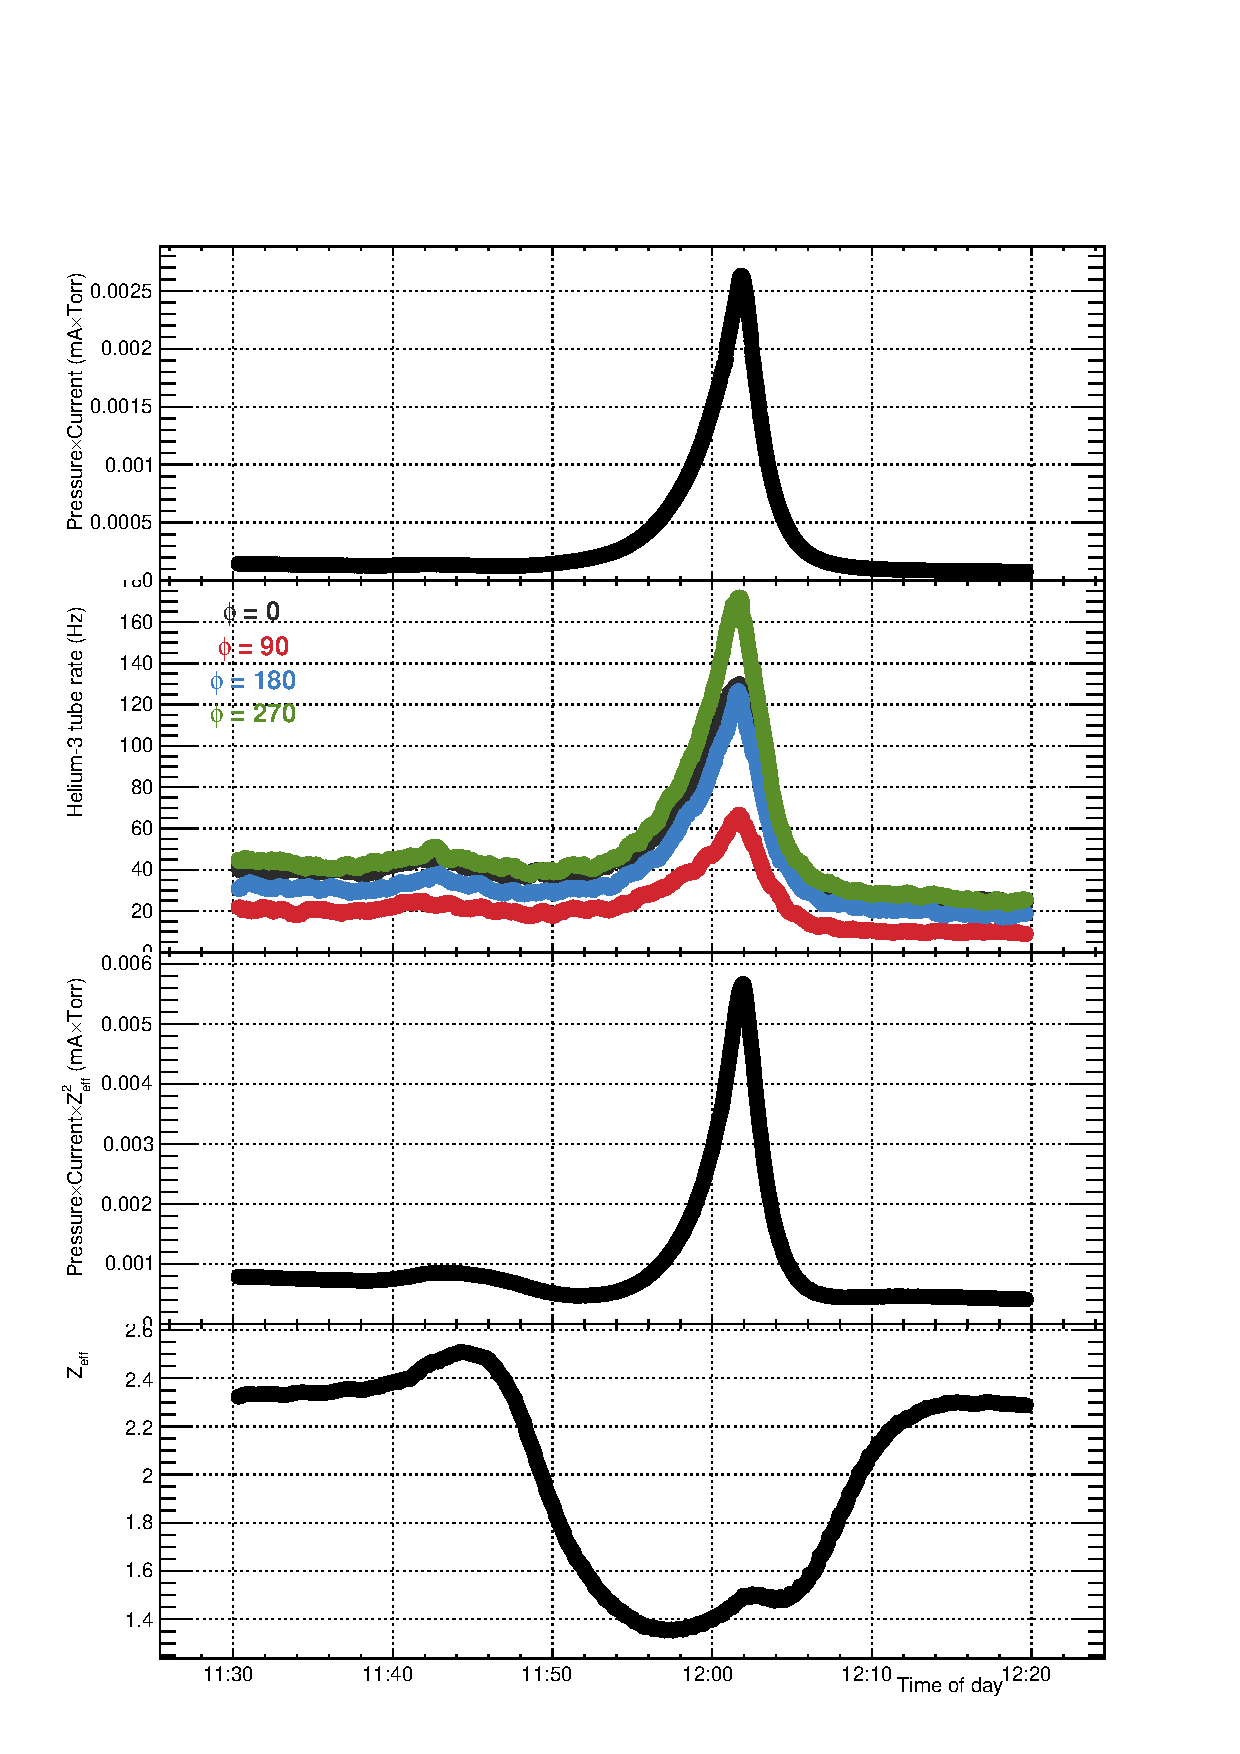
\includegraphics[width=\textwidth]{images/MassSpecCombined}
		\begin{picture}(2,2)
			\put(-100,500){(a)} %1
			\put(-100,380){(b)} %1
			\put(-100,250){(c)} %1
			\put(-100,120){(d)} %1
		\end{picture}
	\caption[Response in \he tubes during vacuum bump run]{Response in \he tubes during vacuum bump run. Data were recorded on May 23, 2016.}	
	\label{fig:rateVsTimeVacuum}
\end{figure}

\begin{figure}
	\centerfloat
		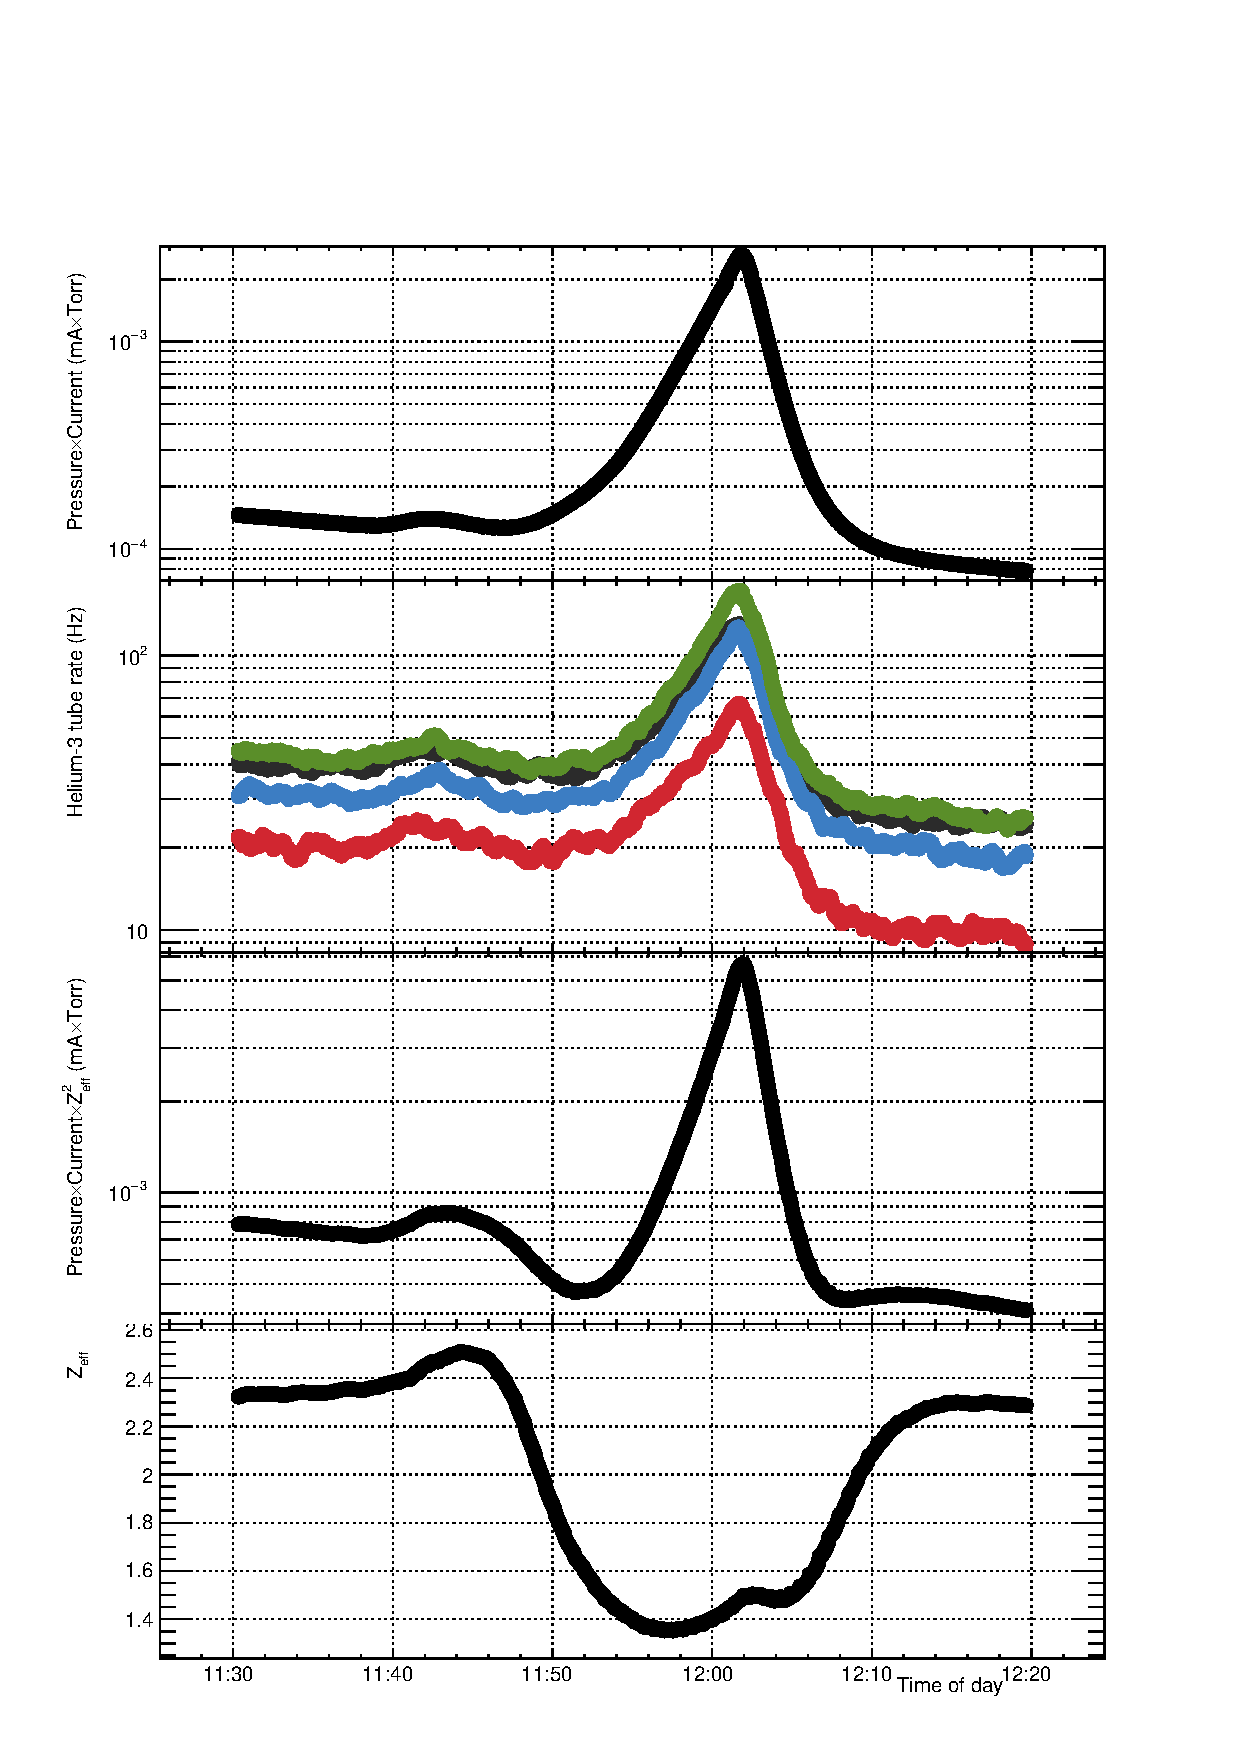
\includegraphics[width=\textwidth]{images/MassSpecCombined_log}
		\begin{picture}(2,2)
			\put(-100,500){(a)} %1
			\put(-100,380){(b)} %1
			\put(-100,250){(c)} %1
			\put(-100,120){(d)} %1
		\end{picture}
	\caption[Response in \he tubes during vacuum bump run, log scale]{Response in \he tubes during vacuum bump run, log scale. Data were recorded on May 23, 2016.}	
	\label{fig:rateVsTimeVacuumlog}
\end{figure}

\paragraph{Smoothing of data}

	Before the analysis of the pressure bumps was done, the data were smoothed using this equation:
\begin{equation}
	{R_{i} = \frac{1}{2n+1}\sum_{j=i-n}^{j=i+n}R_{j}}
\end{equation}
where $R_j$ is the \he tube rate in a one second time bin $j$. This algorithm takes the average of the previous $n$ time bins, the current bin, and the next $n$ bins. For the studies presented here, $n=20$ was used. An example showing the rate in the \he tubes is shown in Fig~\ref{fig:smoothPlot}. This smoothing was done to reduce the fluctuations of the signal. Since this smoothing will reduce the height of the maximum, only the data from the rising portion of the experiment were analysed.

\begin{figure}
	\centering
	\subfigure[Channel 0 ($\phi=0^{\circ}$)]{
		\begin{overpic}[trim={0 0 0 0.5cm},clip, width=0.47\textwidth]{images/SmoothingPlot0}
		\end{overpic}
		\label{fig:smoothPlot0}
	}
	\subfigure[Channel 1 ($\phi=90^{\circ}$)]{
		\begin{overpic}[trim={0 0 0 0.5cm},clip, width=0.47\textwidth]{images/SmoothingPlot1}
		\end{overpic}
		\label{fig:smoothPlot1}
	}
	\subfigure[Channel 2 ($\phi=180^{\circ}$)]{
		\begin{overpic}[trim={0 0 0 0.5cm},clip, width=0.47\textwidth]{images/SmoothingPlot2}
		\end{overpic}
		\label{fig:smoothPlot2}
	}
	\subfigure[Channel 3 ($\phi=270^{\circ}$)]{
		\begin{overpic}[trim={0 0 0 0.5cm},clip, width=0.47\textwidth]{images/SmoothingPlot3}
		\end{overpic}
		\label{fig:smoothPlot3}
	}
	\caption[Smoothing of \he tube data for pressure bump studies]{Smoothing of \he tube data for pressure bump studies where $n=20$. Grey is the unsmoothed data, red is the smoothed data. Data were recorded on May 23, 2016.}
	\label{fig:smoothPlot}
\end{figure}




\subsection{Gas Model Using Beampipe Pressure}

	Initially a simple gas model was used to characterize the response. In this model, it is assumed that the beam-gas cross section is proportional to the pressure in the beampipe. In Fig~\ref{fig:rateVsPressCur}, the rate in the \he tubes is plotted as a function of current times pressure. Only the rising portion of the bumps is plotted, corresponding to time (HH:MM) ranges of 11:40-11:45 for the first bump, and 11:50-12:02 for the second bump. Data are binned in 1 second time bins.


\begin{figure}
	\centering
	\subfigure[Channel 0 ($\phi=0^{\circ}$)]{
		\begin{overpic}[trim={0 0 0 0.5cm},clip, width=0.47\textwidth]{images/HE3_0_withoutMassSpec}
		\end{overpic}
		\label{fig:rateVsPressCur0}
	}
	\subfigure[Channel 1 ($\phi=90^{\circ}$)]{
		\begin{overpic}[trim={0 0 0 0.5cm},clip, width=0.47\textwidth]{images/HE3_1_withoutMassSpec}
		\end{overpic}
		\label{fig:rateVsPressCur1}
	}
	\subfigure[Channel 2 ($\phi=180^{\circ}$)]{
		\begin{overpic}[trim={0 0 0 0.5cm},clip, width=0.47\textwidth]{images/HE3_2_withoutMassSpec}
		\end{overpic}
		\label{fig:rateVsPressCur2}
	}
	\subfigure[Channel 3 ($\phi=270^{\circ}$)]{
		\begin{overpic}[trim={0 0 0 0.5cm},clip, width=0.47\textwidth]{images/HE3_3_withoutMassSpec}
		\end{overpic}
		\label{fig:rateVsPressCur3}
	}
	\caption[Rate in \he tubes vs pressure times current in LER beam]{Rate in \he tubes vs pressure times current in LER beam. Blue corresponds to the larger pressure increase occurring from 11:50 to 12:02 and orange corresponds to the small pressure increase occurring from 11:40 to 11:45.}	
	\label{fig:rateVsPressCur}
\end{figure}




	As evident from Fig~\ref{fig:rateVsPressCur}, the response due to the first bump is quite different from the response due to the second bump. The simple gas model that assumes that the beam-gas rate is proportional to $P\cdot I$ does not adequately describe what is happening in this data. A more complex gas model is necessary.



\subsection{Gas Model Using Mass Spectrum Data}
\label{sec:massSpec}


	The elastic and inelastic cross sections of beam particles interacting with gas in the beampipe are given by Eqns~\ref{eqn:coulomb} and~\ref{eqn:brems}. Both cross sections are approximately proportional to $Z^2$, where $Z$ is the number of protons in the target. If the gas composition in the beampipe does not change, $Z^2$ will be constant, and the change in beampipe pressure alone is sufficient to determine the beam-gas cross section. If it is known that the gas composition is changing, however, simply using pressure will produce different responses as seen in Fig~\ref{fig:rateVsPressCur}. Therefore a more complex gas model is necessary.


\subsubsection{Mass Spectrum Fit}

	The SuperKEKB collider has two residual gas analysers (RGAs) on the LER beampipe, located at D02 and D06 (see Fig~\ref{fig:SKBVac}). These devices are simple mass spectrometers, which measure the partial pressure for mass-to-charge ratio (m/z) values from 1 to 50 (m is number of nucleons in a molecule `fragment', z is the charge of the `fragment', so m/z has no units). Using this information, it is possible to infer the composition of the gas in the beampipe. 


\begin{table}
	\centering
	\begin{tabular}{ cc }
		Molecule Name	& Number of protons	\\	\hline \hline
		$H_2$		& 2		\\	
		$D_2$		& 2		\\	
		$DH$		& 2		\\	
		$H_{2}O$	& 10		\\	
		$H_{3}N$	& 10		\\	
		$CH_4$		& 10		\\	
		$CO$		& 14		\\	
		$C_{2}H_4$	& 16		\\	
		$Ar$		& 18		\\	
		$C_{2}H_6$	& 18		\\	
		$CO_2$		& 22		\\	
		$C_{3}H_4$	& 22		\\	
		$C_{3}H_6$	& 24		\\	
		$C_{3}H_8$	& 26		\\ \hline
	\end{tabular}
	\caption[Molecules used in fit to RGA data]{Molecules used in fit to RGA data.}
	\label{tab:Molecules}
\end{table}


	Using mass spectra data taken from the National Institute of Standards and Technology (NIST) database \cite{nistMassSpec}, the spectra of various molecules were fit to the data measured by the RGA. A list of the gases used in the fit is given in Table~\ref{tab:Molecules}, and example spectra of the most prominent molecules present in the beampipe are shown in Fig~\ref{fig:ExampleMassSpecs}. 

The mass spectrum measured by the RGA is a linear sum of the mass spectra from all the gases that make up the gas mixture in the beampipe \cite{MassSpecBook}:
\begin{equation}
	{\vec{S}^{\mathrm{Measured}} = \sum_{i=1}^{n_{\mathrm{molecules}}}p_{i}\vec{S}^{\mathrm{Template}}_{i} \equiv \textbf{S}^{\mathrm{Template}}\vec{p}}
\end{equation}
where $\vec{S}^{\mathrm{Measured}}$ is a vector containing the data measured by the RGA (the partial pressure for m/z from 1 to 50, shown in black in Fig~\ref{fig:mSpecFit}), $\vec{S}_{i}^{\mathrm{Template}}$ is a vector containing the spectrum of a molecular species spectrum (for example, H$_2$O as in Fig~\ref{fig:exampleH2O}), and $p_{i}$ is the partial pressure of that species, which is extracted from the fit. This is equivalent to a matrix equation, where $\vec{p}$ is a vector containing the partial pressure of each gas species, and $\textbf{S}^{\mathrm{Template}}$ is a matrix with the mass spectra vectors $\vec{S}_{i}^{\mathrm{Template}}$ as the columns. To find the partial pressure of each gas species, a least squares analysis is used, the solution to which is \cite{LinAlg}:
\begin{equation}
	{\vec{p}_{\mathrm{min}}=\left ( [\textbf{S}^{\mathrm{Template}}]^{T}\textbf{S}^{\mathrm{Template}} \right )^{-1}[\textbf{S}^{\mathrm{Template}}]^{T}\vec{S}^{\mathrm{Measured}}}
	\label{eqn:LSQ}
\end{equation}
Solving this gives the partial pressure of each gas species in the beampipe at that moment. 



Uncertainties are estimated by taking the diagonal entries of~\cite{LinAlg2}:

\begin{equation}
		{\pmb{\sigma_{\vec{p}_{\mathrm{min}}}^{2}}=\left( [\textbf{S}^{\mathrm{Template}}]^{T}\textbf{S}^{\mathrm{Template}} \right )^{-1}\sigma^{2}}\\
\label{eqn:FitUncer}
\end{equation}
where 
\begin{equation}
		{\sigma^2=|\textbf{S}^{\mathrm{Template}}\vec{p_{\mathrm{min}}}-\vec{S}^{\mathrm{Measured}}|^2}
\end{equation}


Plots showing the result of this fit for a single time bin are shown in Fig~\ref{fig:MassSpecFitting}. By repeating this procedure for each time bin, it is possible to see how the gas mixture in the beampipe changes.

\begin{figure}
	\centering
	\subfigure[H$_2$]{
		\begin{overpic}[trim={0 0 0 0.75cm},clip, width=\textwidth]{images/H2_MassSpec}
		\end{overpic}
		\label{fig:exampleH2}
	}
	\subfigure[CO]{
		\begin{overpic}[trim={0 0 0 0.75cm},clip, width=\textwidth]{images/CO_MassSpec}
		\end{overpic}
		\label{fig:exampleCO}
	}
	\subfigure[H$_2$O]{
		\begin{overpic}[trim={0 0 0 0.75cm},clip, width=\textwidth]{images/H2O_MassSpec}
		\end{overpic}
		\label{fig:exampleH2O}
	}
	\caption[Example mass spectra]{Example mass spectra for the most prominent molecules present in the beampipe~\cite{nistMassSpec}.}
	\label{fig:ExampleMassSpecs}
\end{figure}



	
\begin{figure}
	\centering
	\subfigure[Mass spectrum with fit. Black is data, red is fit]{
		\begin{overpic}[trim={0 0 0 0.75cm},clip, width=\textwidth]{images/MassSpecwFit}
		\end{overpic}
		\label{fig:mSpecFit}
	}
	\subfigure[Partial pressure of gas species]{
		\begin{overpic}[trim={0 0 0 0.75cm},clip, width=\textwidth]{images/GasSpecies}
		\end{overpic}
		\label{fig:gasSpecies}
	}
	\caption[Mass spectrum fit examples]{Mass spectrum fit examples. Uncertainties are obtained from Eqn~\ref{eqn:FitUncer}.}	
	\label{fig:MassSpecFitting}
\end{figure}

\subsubsection{Gas Model}

In \S~\ref{sec:beamGas}, it is shown that the cross section for both elastic and inelastic collisions with gas is proportional to the square of the number of protons in the gas molecule, $Z^2$. Using the mass spectrum fitting procedure, an effective $Z$ can be defined as the weighted sum of $Z$ for each gas molecule:
\begin{equation}
	{Z_{\mathrm{eff}}^2 = \frac{\sum_{i=1}^{n_{\mathrm{atoms}}}p_{i}Z_{i}^2}{\sum_{i}^{n_{\mathrm{atoms}}}p_i}}
	\label{eqn:ZEFF}
\end{equation}
where $Z_{i}$ is the number of protons in each gas species (see Table~\ref{tab:Molecules}) and $p_i$ is the partial pressure of each gas species. Fig~\ref{fig:rateVsTimeVacuum}(d) shows a plot of how $Z_{\mathrm{eff}}$ changes over the course of a beam bump run. It is clear that the gas composition changes over the course of the run. 

	$Z_{\mathrm{eff}}$ is then the atomic number of a pure gas that would produce the same background as the gas mixture in the beampipe.


	$P\cdot I$ is then weighted by $Z_{\mathrm{eff}}^2$, as shown in Fig~\ref{fig:rateVsTimeVacuum}(c) and Fig~\ref {fig:rateVsTimeVacuumlog}(c). A plot of the rate in the \he tubes vs $P\cdot I \cdot Z_{\mathrm{eff}}^2$ is shown in Fig~\ref{fig:rateVsPressCurWeight}. It can be seen from this figure that the slope of the response to both bumps is very similar, demonstrating that multiplying by $Z_{\mathrm{eff}}^2$ explains the problem of the different slopes in Fig~\ref{fig:rateVsPressCur}.


\begin{figure}
	\centering
	\subfigure[Channel 0 ($\phi=0^{\circ}$)]{
		\begin{overpic}[trim={0 0 0 0.5cm},clip, width=0.47\textwidth]{images/HE3_0_withMassSpec}
		\end{overpic}
		\label{fig:rateVsPressCurWeight0}
	}
	\subfigure[Channel 1 ($\phi=90^{\circ}$)]{
		\begin{overpic}[trim={0 0 0 0.5cm},clip, width=0.47\textwidth]{images/HE3_1_withMassSpec}
		\end{overpic}
		\label{fig:rateVsPressCurWeight1}
	}
	\subfigure[Channel 2 ($\phi=180^{\circ}$)]{
		\begin{overpic}[trim={0 0 0 0.5cm},clip, width=0.47\textwidth]{images/HE3_2_withMassSpec}
		\end{overpic}
		\label{fig:rateVsPressCurWeight2}
	}
	\subfigure[Channel 3 ($\phi=270^{\circ}$)]{
		\begin{overpic}[trim={0 0 0 0.5cm},clip, width=0.47\textwidth]{images/HE3_3_withMassSpec}
		\end{overpic}
		\label{fig:rateVsPressCurWeight3}
	}
	\caption[Rate in \he tubes vs pressure times current weighted by $Z_{\mathrm{eff}}^2$ in LER beam]{Rate in \he tubes vs pressure times current weighted by $Z_{\mathrm{eff}}^2$ in LER beam. Blue corresponds to  the larger pressure increase occurring from 11:50 to 12:02 and orange corresponds to the small pressure increase occurring from 11:40 to 11:45 (HH:MM).}	
	\label{fig:rateVsPressCurWeight}
\end{figure}


\subsection{Slope Ratio}

	In order to quantify the improvement that the mass spectrum based gas model provides, a quantity called the slope ratio is defined:
\begin{equation}
	{\mathrm{Slope~Ratio} = \frac{m_{2}}{m_{1}}}
\end{equation}
where $m_{1}$ is the slope of a line fit to the rate vs $P\cdot I$ (weighted or unweighted) of the first bump, and $m_{2}$ is the same for the second bump. The more accurate the gas model, the closer the slope ratio will be to 1. The slope ratio for each \he tube is shown in Fig~\ref{fig:slopeRatio} for when $P\cdot I$ is weighted by $Z_{\mathrm{eff}}^2$, and when it is not weighted.


\begin{figure}
	\centerfloat
		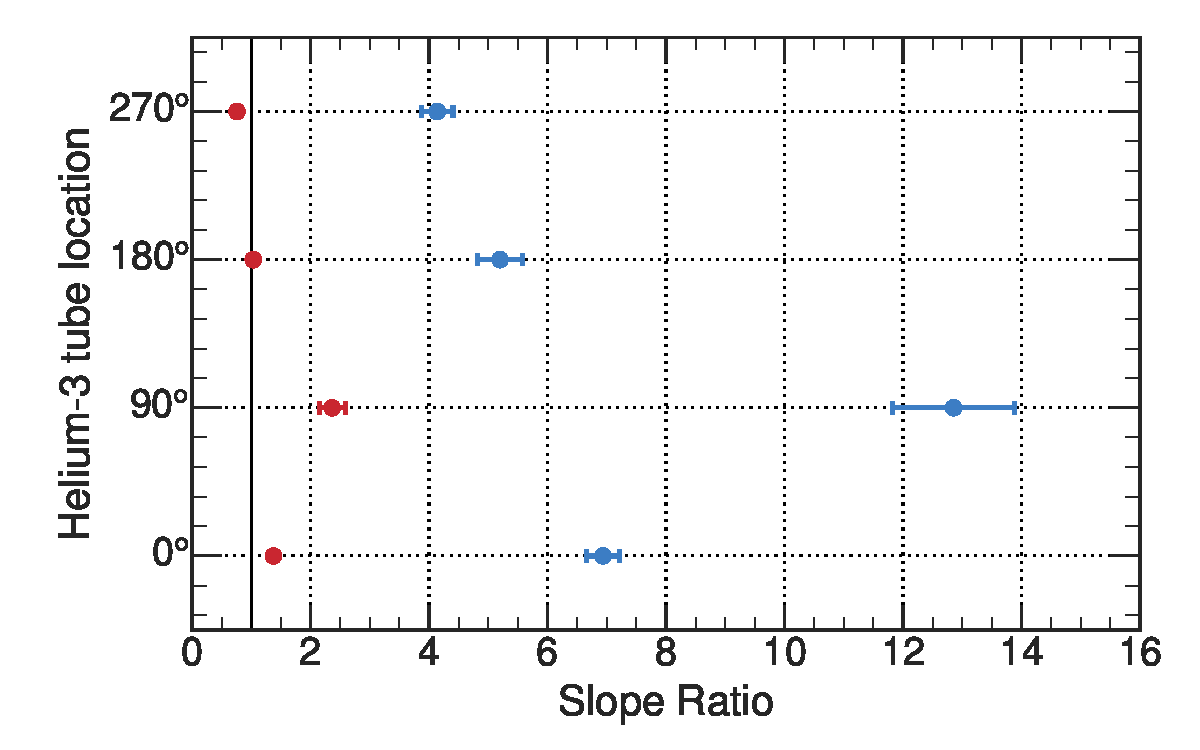
\includegraphics[width=\textwidth]{images/SlopeRatioPlot_He3}
	\caption[Comparison of gas models with slope ratio]{Comparison of gas models with slope ratio. Red is the ratio of the slopes from the $P\cdot I\cdot Z_{\mathrm{eff}}^2$ model and blue is ratio of the slopes from the $P\cdot I$ gas model. The black line is at a slope ratio of one.}	
	\label{fig:slopeRatio}
\end{figure}

As shown in the figure, including $Z_{\mathrm{eff}}$ in the gas model produces a significant improvement in understanding the response to the vacuum bump, indicating that a difference in the gas composition is mainly responsible for the different rate vs $P\cdot I$ dependence for the two bumps. This shows that the rate actually depends on $P\cdot I\cdot Z_{\mathrm{eff}}^2$. Note that the \he tubes at $\phi=0^{\circ}$ and 90$^{\circ}$ are not as close to 1 as 180$^{\circ}$ and 270$^{\circ}$, but are still much improved over the $P\cdot I$ model. Note that Fig~\ref{fig:rateVsPressCurWeight1} shows some systematic effect in the tube 1 (90$^{\circ}$) rates for the second bump, with a significant non-constant slope relative to the others, resulting in a much larger deviation in the slope ratio.


%------------------------------------------------------------------------------------------------



\section{Touschek experiments}
\label{sec:TousExp}

	In order to separate the beam-gas and beam-beam component of the \he tube rate during the beam size scans, the rate is fit to this function:
\begin{equation}
	{R_{^{3}\mathrm{He tube}} = c_{\mathrm{gas}}\cdot P\cdot I\cdot Z_{\mathrm{eff}}^{2}+c_{\mathrm{T}}\cdot \frac{I^{2}}{N_{\mathrm{Bunch}}\cdot\sigma_{y}}}
	\label{eqn:TousFit}
\end{equation}
where $P$ is the pressure in the beampipe, $I$ is the beam current, $Z_{\mathrm{eff}}$ is the atomic number of the beampipe gas, $\sigma_{y}$ is the size of the beam, and $c_{\mathrm{gas}}$ and $c_{\mathrm{T}}$ are the fit parameters. Fig~\ref{fig:tousZef} shows how $Z_{\mathrm{eff}}$ changes during the beam size runs, showing the importance of including it in the fit. For the LER, the value of $Z_{\mathrm{eff}}$ measured at D02 is used. This technique is described in detail in \S~\ref{sec:PBump}. The HER has no RGA, and therefore it is not possible to determine the value of $Z_{\mathrm{eff}}$, so a value of 1 is assumed. The $P_{\mathrm{scale}}$ factor used in the simulation scaling (see Chapter ~\ref{chap:Sim}) is 1.


\begin{figure}
	\centerfloat
		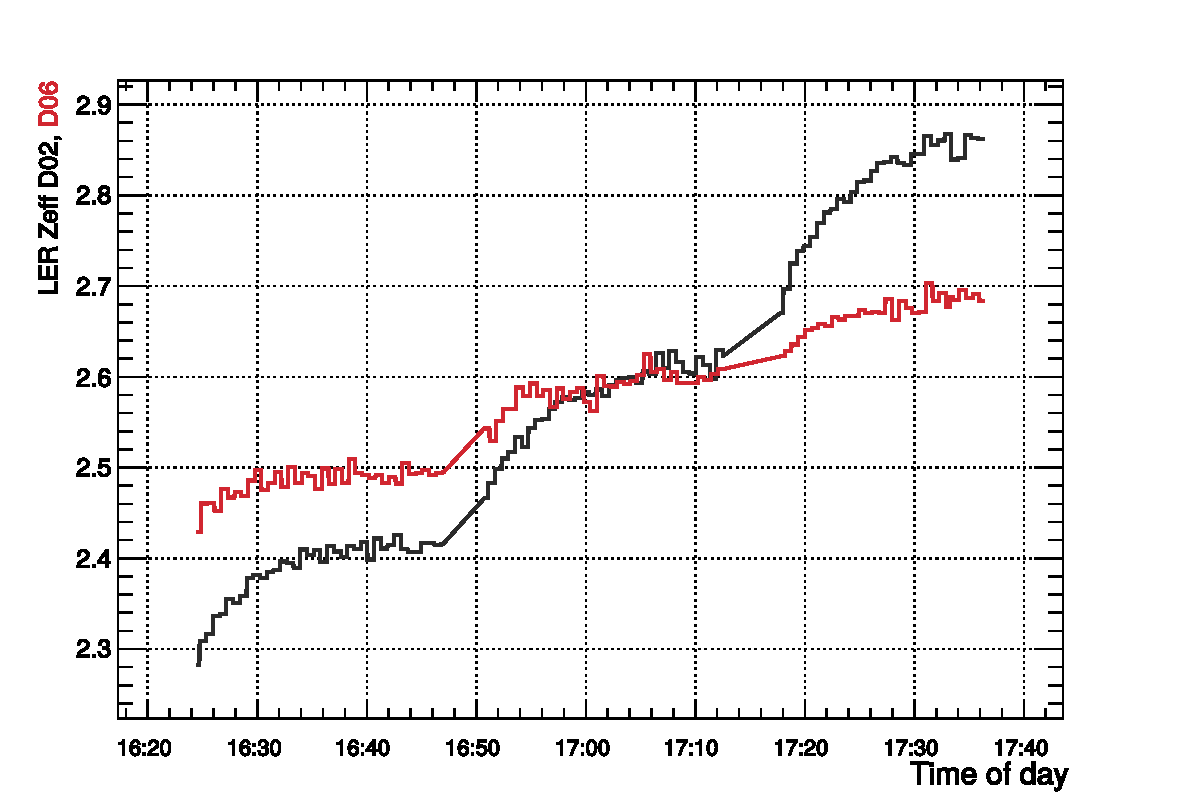
\includegraphics[width=\textwidth]{images/Zeff}
	\caption[$Z_{\mathrm{eff}}$ during LER beam size runs]{$Z_{\mathrm{eff}}$ during LER beam size runs. Data were recorded on May 17, 2016.}	
	\label{fig:tousZef}
\end{figure}

The results of this fit for data and simulation for LER and HER are shown in Figs~\ref{fig:LERTous10},~\ref{fig:LERTous11},~\ref{fig:LERTous12},~\ref{fig:LERTous13}, and~\ref{fig:HERTous10},~\ref{fig:HERTous11},~\ref{fig:HERTous12},~\ref{fig:HERTous13} respectively. The data are divided into three runs, each with five subruns. The runs occurred at different injection currents, and the subruns each had different beam sizes. In these figures, the black points are the average measured \he tube rate in each bin. The Touschek component, in green, is given by:
\begin{equation}
	R_{\mathrm{T}} = c_{\mathrm{T}}\cdot \frac{I^{2}}{N_{\mathrm{Bunch}}\cdot\sigma_{y}}
\end{equation}
and the beam-gas component, in blue, is given by:
\begin{equation}
	R_{\mathrm{gas}} = c_{\mathrm{gas}}\cdot P\cdot I\cdot Z_{\mathrm{eff}}^{2}
\end{equation}
The error bars shown are the RMS of the \he tube rate for that bin. The pressure in the beampipe is changing over the course of the experiments and is included in the fit, but for simplicity is not shown in the figures. The values produced by the fit can be found in Table~\ref{tab:FitPars}, and $\chi^2$ and number of degrees of freedom (ndf) are in Table~\ref{tab:ChiNDF}. Note that only statistical errors and fit parameters uncertainties are included in the $\chi^2$ calculation. If the systematic errors are included, $\chi^2$ becomes significantly smaller.


\begin{sidewaystable}
    \centering
    \begin{tabular}{cc|cc|cc|cccc}
	&		&	 \multicolumn{2}{c}{Data}			&	 \multicolumn{2}{c}{Simulation – Initial Scaling} 			&	 \multicolumn{2}{c}{Simulation – Corrected Scaling}  	 		\\	
	&	 	&	 c$_{\mathrm{gas}}$	&	 c$_{T}$	&	 c$_{\mathrm{gas}}$	&	 c$_{T}$ 	&	 c$_{\mathrm{gas}}$	&	 c$_{T}$ 	\\	
	&	Channel 	&	  [$Hz/(mA\cdot Pa)$]	&	 [$Hz\cdot\mu m/mA^{2}$]	&	 [$Hz/(mA\cdot Pa)$]	&	 [$Hz\cdot\mu m/mA^{2}$]  	&	  [$Hz/(mA\cdot Pa)$]	&	 [$Hz\cdot\mu m/mA^{2}$]  	\\	\hline \hline
LER	&	 0	&	 6500$\pm$400	&	 16.4$\pm$0.6	&	 3120.4$\pm$5	&	 8.028$\pm$0.007	&	 2963$\pm$5	&	 8.026$\pm$0.006	\\	
	&	 1	&	 3400$\pm$200	&	 8.1$\pm$0.3	&	 2401$\pm$4	&	 5.098$\pm$0.005	&	 2281$\pm$4	&	 5.097$\pm$0.005	\\	
	&	 2	&	 5700$\pm$300	&	 13.4$\pm$0.4	&	 1901$\pm$3	&	 4.653$\pm$0.004	&	 1806$\pm$3	&	 4.651$\pm$0.004	\\	
	&	 3	&	 8000$\pm$400	&	 18.1$\pm$0.5	&	 4076$\pm$7	&	 9.0245$\pm$0.008	&	 3872$\pm$7	&	 9.022$\pm$0.008	\\	\hline
HER	&	0	&	 (241$\pm$5)$\times10^{3}$	&	 0.21$\pm$0.04	&	 1750$\pm$30	&	 0.1963$\pm$0.0002 	&	 (151$\pm$1.5)$\times10^{3}$	&	 0.140$\pm$0.013	\\	
	&	1	&	 (108$\pm$4)$\times10^{3}$	&	 0.13$\pm$0.03	&	 1280.9$\pm$17	&	 0.0944$\pm$0.00014	&	 (104$\pm$1.0)$\times10^{3}$	&	 0.0507$\pm$0.009	\\	
	&	2	&	 (175$\pm$3)$\times10^{3}$	&	 0.21$\pm$0.03	&	 1030$\pm$15	&	 0.09052$\pm$0.00012	&	 (88.5$\pm$0.9)$\times10^{3}$ 	&	 0.0564$\pm$0.007	\\	
	&	3	&	 (241$\pm$4)$\times10^{3}$	&	 0.23$\pm$0.03	&	 2411$\pm$40	&	 0.26543$\pm$0.0003 	&	 (213$\pm$2.2)$\times10^{3}$	&	 0.189$\pm$0.018 	\\	\hline

    \end{tabular}
    \caption[Fit parameters associated with Figs~\ref{fig:LERTous10} to~\ref{fig:HERTous23}]{Fit parameters associated with Figs~\ref{fig:LERTous10} to~\ref{fig:HERTous23}. $\chi^2$ and ndf can be found in Table~\ref{tab:ChiNDF}.}
    \label{tab:FitPars}
\end{sidewaystable}


\begin{sidewaystable}
    \centering
    \begin{tabular}{cc|cc|cc|cccc}
	&		&	 \multicolumn{2}{c}{Data}			&	 \multicolumn{2}{c}{Simulation – Initial Scaling} 			&	 \multicolumn{2}{c}{Simulation – Corrected Scaling}  			\\	
	&	Channel 	&	$\chi^2$	&	ndf	&	$\chi^2$	&	ndf	&	$\chi^2$	&	ndf	\\	\hline \hline
LER	&	 0	&	141.57	&	12	&	23.206	&	12	&	21.504	&	12	\\	
	&	 1	&	85.587	&	12	&	30.489	&	12	&	28.446	&	12	\\	
	&	 2	&	106.37	&	12	&	24.988	&	12	&	23.192	&	12	\\	
	&	 3	&	116.51	&	12	&	28.789	&	12	&	26.819	&	12	\\	\hline
HER	&	0	&	7.7796	&	12	&	3.8825	&	12	&	24.408	&	12	\\	
	&	1	&	10.176	&	12	&	4.9767	&	12	&	22.25	&	12	\\	
	&	2	&	6.2589	&	12	&	4.333	&	12	&	21.303	&	12	\\	
	&	3	&	7.0256	&	12	&	3.8597	&	12	&	22.24	&	12	\\	\hline
    \end{tabular}
    \caption[$\chi^2$ and ndf for Figs~\ref{fig:LERTous10} to~\ref{fig:HERTous23}]{$\chi^2$ and ndf for Figs~\ref{fig:LERTous10} to~\ref{fig:HERTous23}. Note that only the statistical errors and fit parameter uncertainties are included in the calculation of $\chi^2$.}
    \label{tab:ChiNDF}
\end{sidewaystable}



\begin{figure}
	\centerfloat
		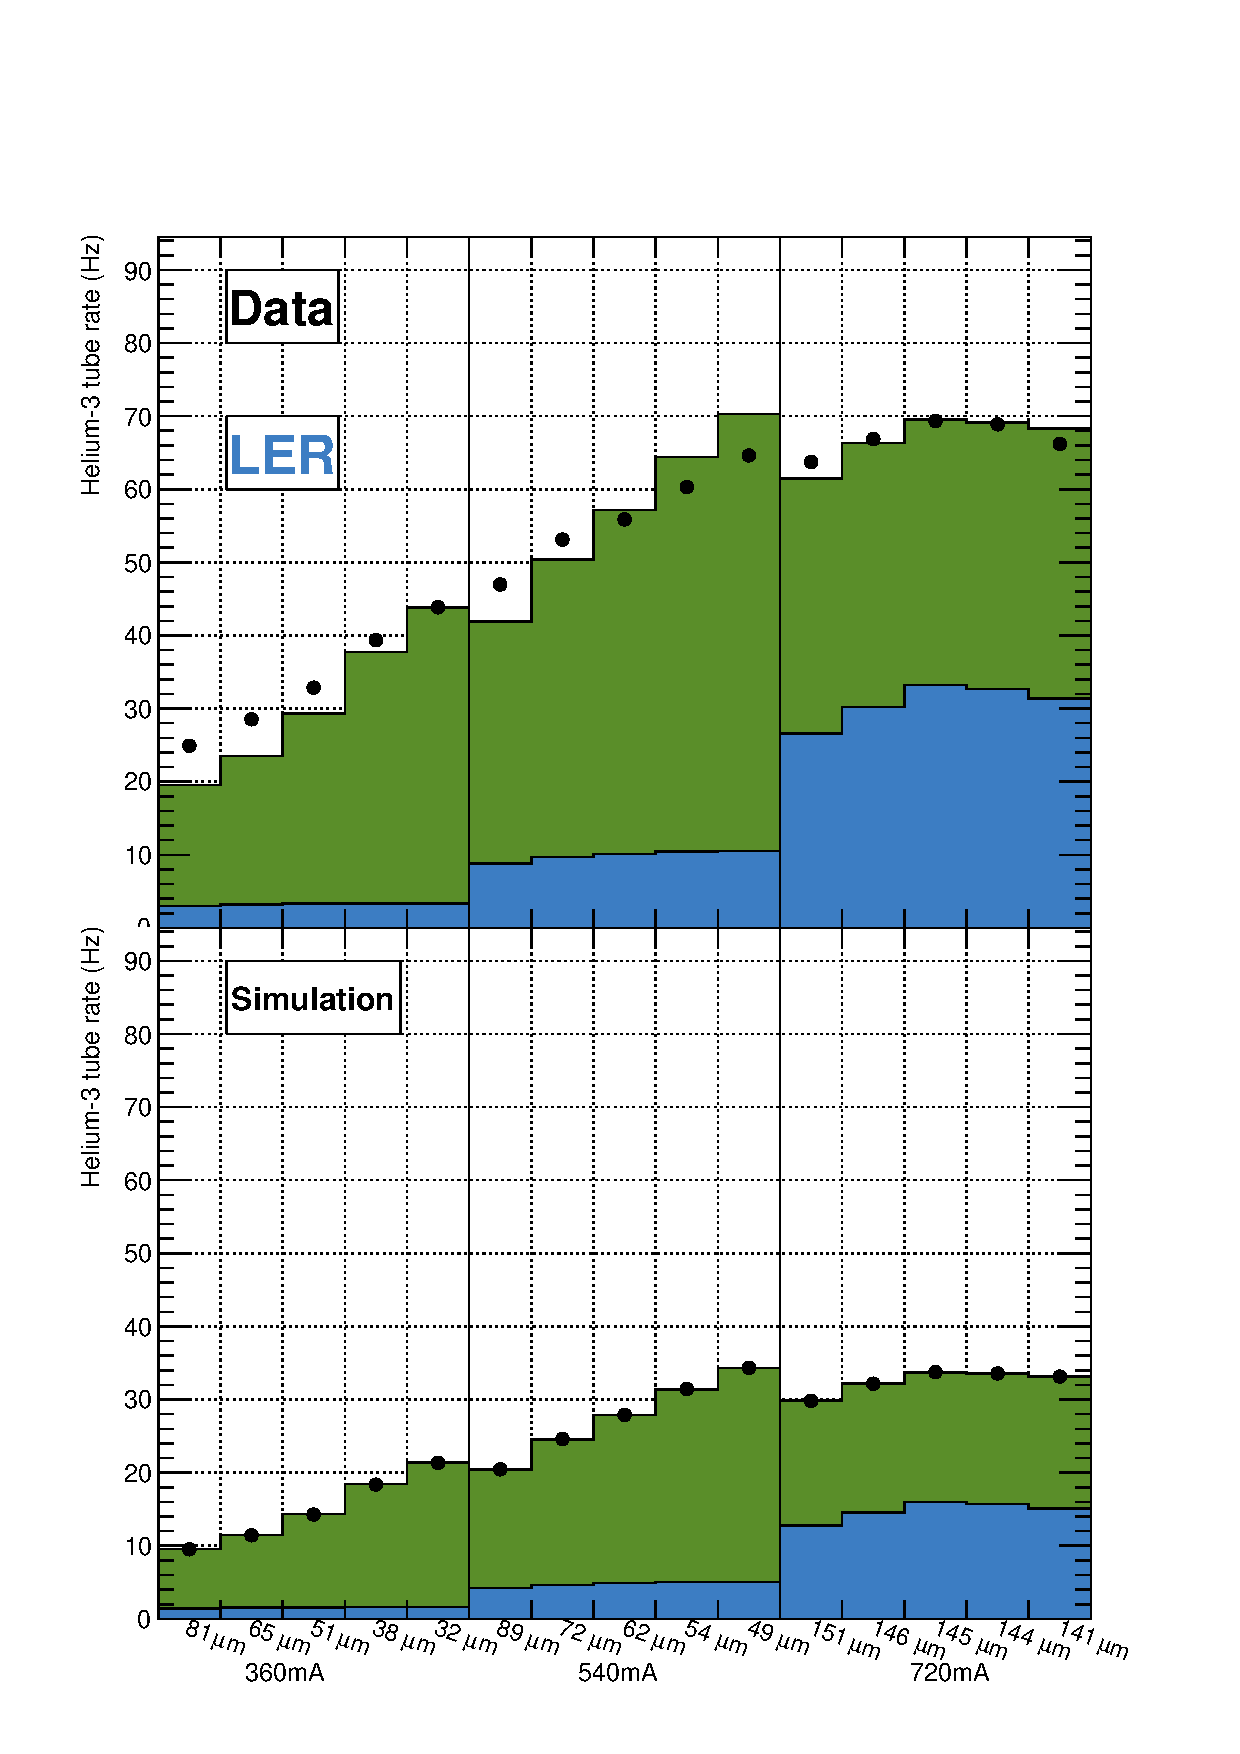
\includegraphics[width=\textwidth]{images/LERTousFirstPass_0}
		\begin{picture}(2,2)
			\put(-100,260){\thicklines\circle{10}} %1
			\put(-120,240){\thicklines\circle{10}}  %2
			\put(-100,220){\thicklines\circle{10}}  %3
			\put(-80,240){\thicklines\circle*{10}}   %0
			\put(-104, 237){$\phi$}  
		\end{picture}
	\caption[Result of fit for Touschek experiments, LER, channel 0]{Result of fit for Touschek experiments, LER, channel 0. Green is the beam-beam component, blue is the beam-gas component, and black is the rate measured in \he tube channel 0. Error bars are the standard deviation of the mean of the rate in that bin and are too small to be seen on this scale.}	
	\label{fig:LERTous10}
\end{figure}


\begin{figure}
	\centerfloat
		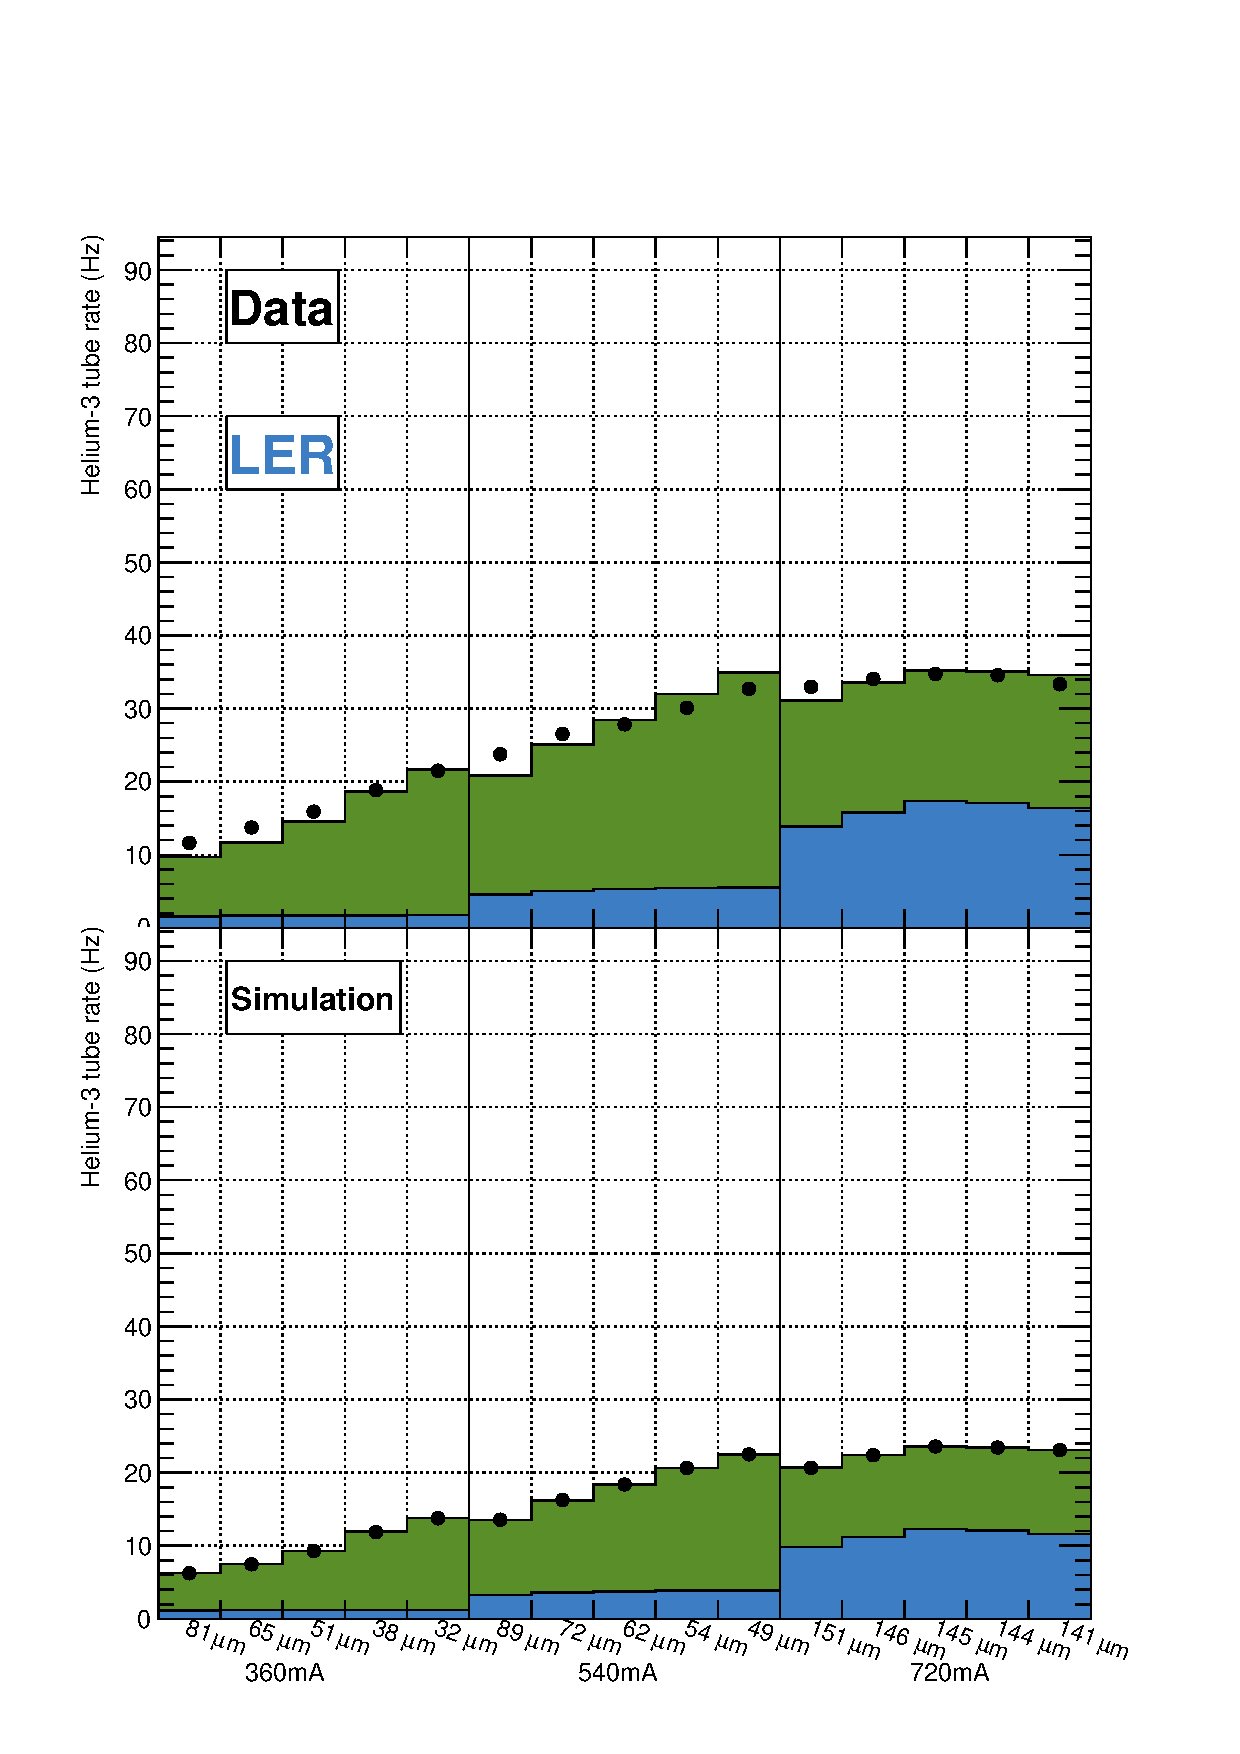
\includegraphics[width=\textwidth]{images/LERTousFirstPass_1}
		\begin{picture}(2,2)
			\put(-100,260){\thicklines\circle*{10}} %1
			\put(-120,240){\thicklines\circle{10}}  %2
			\put(-100,220){\thicklines\circle{10}}  %3
			\put(-80,240){\thicklines\circle{10}}   %0
			\put(-104, 237){$\phi$}  
		\end{picture}
	\caption[Result of fit for Touschek experiments, LER, channel 1]{Result of fit for Touschek experiments, LER, channel 1. Green is the beam-beam component, blue is the beam-gas component, and black is the rate measured in \he tube channel 1. Error bars are the standard deviation of the mean of the rate in that bin and are too small to be seen on this scale.}	
	\label{fig:LERTous11}
\end{figure}

\begin{figure}
	\centerfloat
		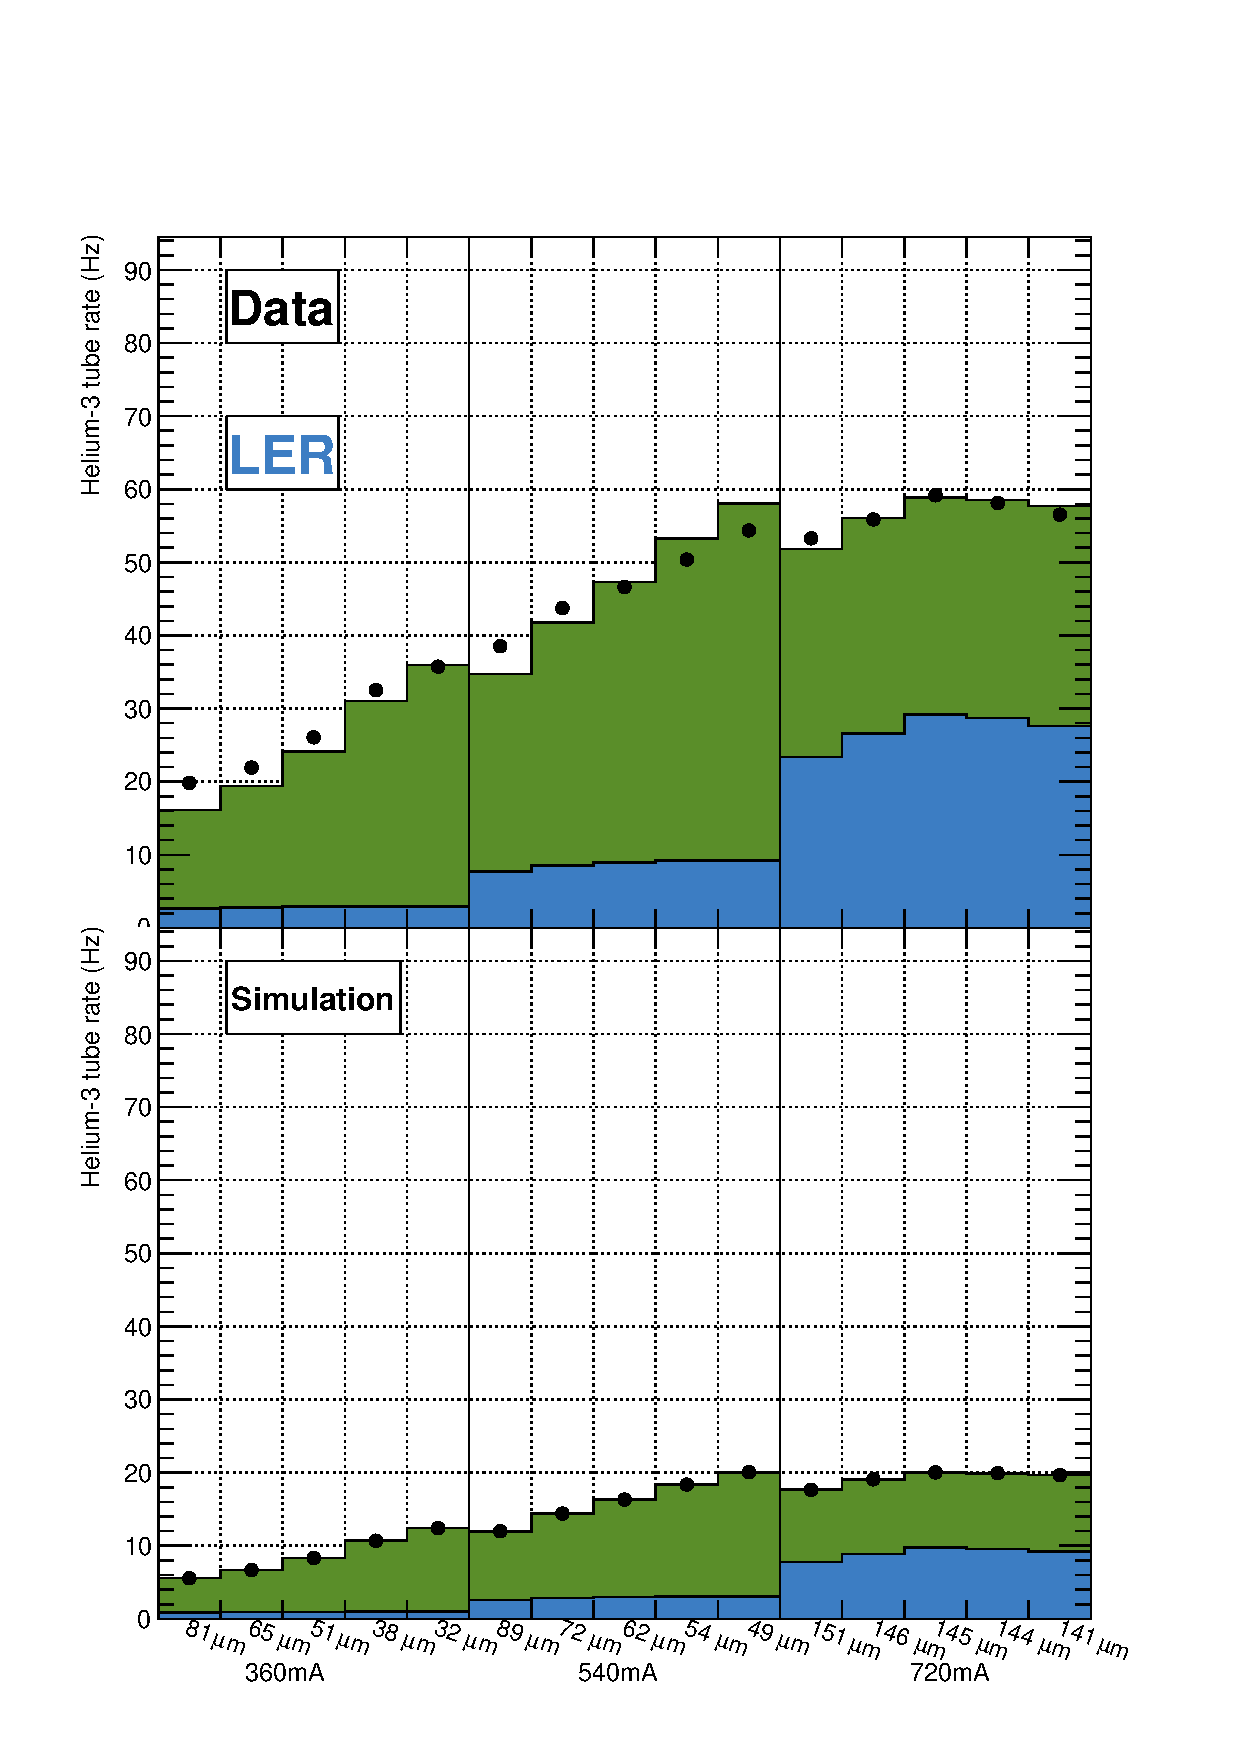
\includegraphics[width=\textwidth]{images/LERTousFirstPass_2}	
		\begin{picture}(2,2)
			\put(-100,260){\thicklines\circle{10}} %1
			\put(-120,240){\thicklines\circle*{10}}  %2
			\put(-100,220){\thicklines\circle{10}}  %3
			\put(-80,240){\thicklines\circle{10}}   %0
			\put(-104, 237){$\phi$}  
		\end{picture}
	\caption[Result of fit for Touschek experiments, LER, channel 2]{Result of fit for Touschek experiments, LER, channel 2. Green is the beam-beam component, blue is the beam-gas component, and black is the rate measured in \he tube channel 2. Error bars are the standard deviation of the mean of the rate in that bin and are too small to be seen on this scale.}	
	\label{fig:LERTous12}
\end{figure}

\begin{figure}
	\centerfloat
		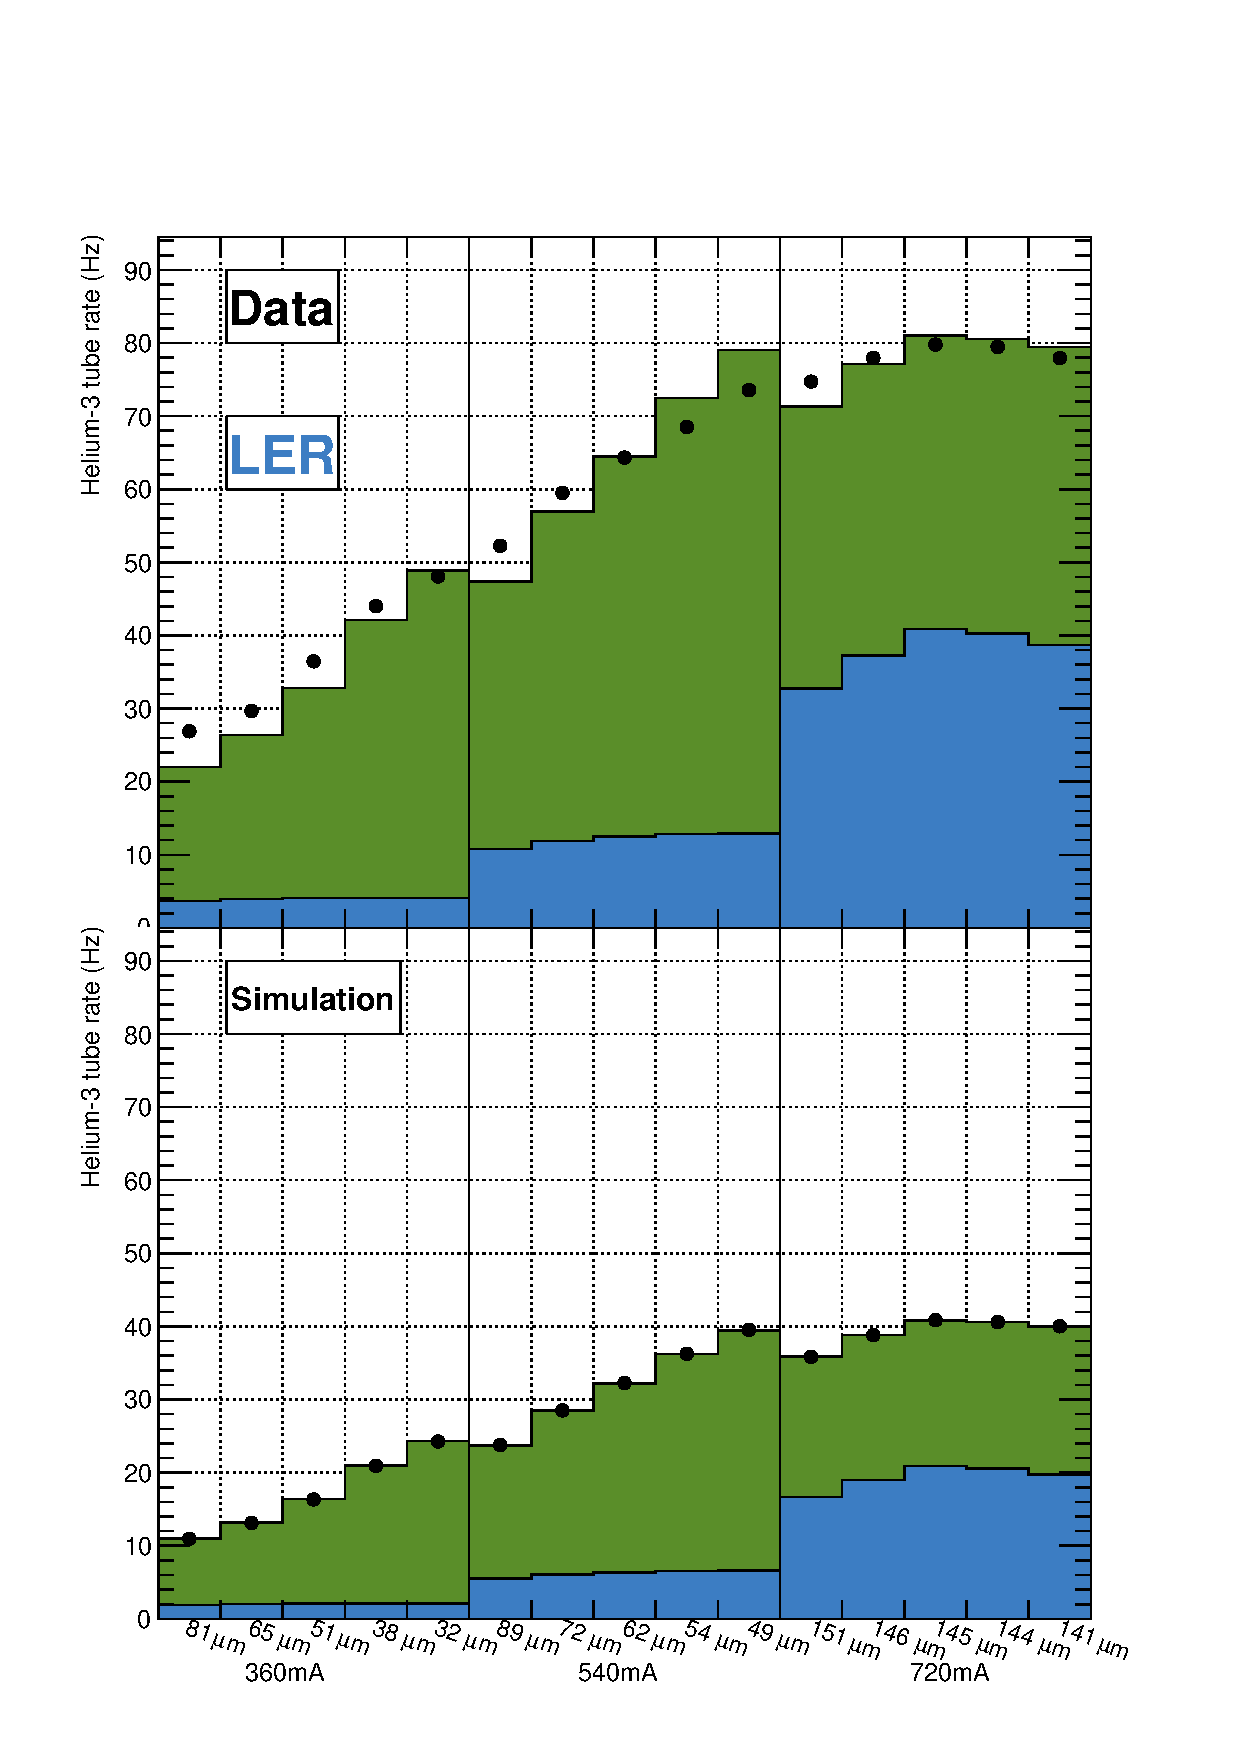
\includegraphics[width=\textwidth]{images/LERTousFirstPass_3}
		\begin{picture}(2,2)
			\put(-100,260){\thicklines\circle{10}} %1
			\put(-120,240){\thicklines\circle{10}}  %2
			\put(-100,220){\thicklines\circle*{10}}  %3
			\put(-80,240){\thicklines\circle{10}}   %0
			\put(-104, 237){$\phi$}  
		\end{picture}
	\caption[Result of fit for Touschek experiments, LER, channel 3]{Result of fit for Touschek experiments, LER, channel 3. Green is the beam-beam component, blue is the beam-gas component, and black is the rate measured in \he tube channel 3. Error bars are the standard deviation of the mean of the rate in that bin.}	
	\label{fig:LERTous13}
\end{figure}





\begin{figure}
	\centerfloat
		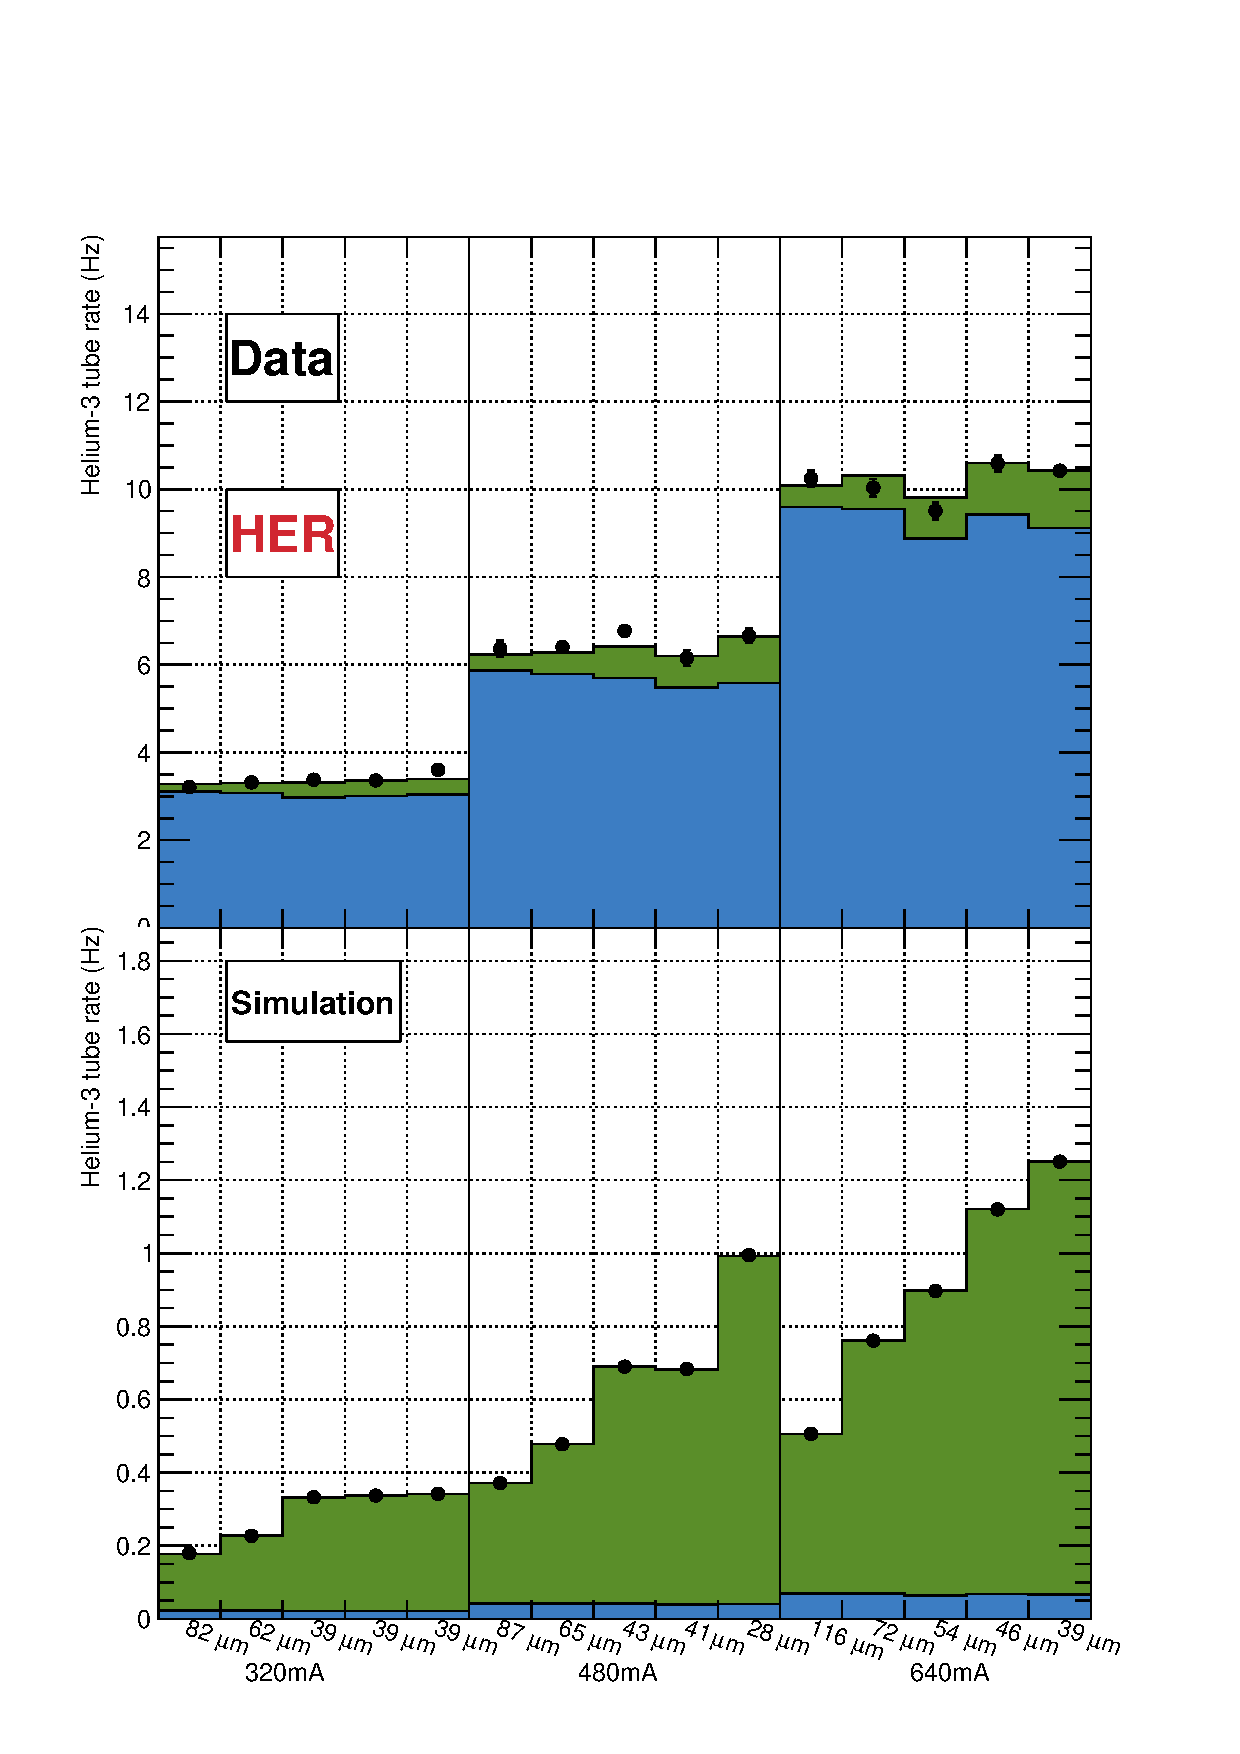
\includegraphics[width=\textwidth]{images/HERTousFirstPass_0}
		\begin{picture}(2,2)
			\put(-100,260){\thicklines\circle{10}} %1
			\put(-120,240){\thicklines\circle{10}}  %2
			\put(-100,220){\thicklines\circle{10}}  %3
			\put(-80,240){\thicklines\circle*{10}}   %0
			\put(-104, 237){$\phi$}  
		\end{picture}
	\caption[Result of fit for Touschek experiments, HER, channel 0]{Result of fit for Touschek experiments, HER, channel 0. Green is the beam-beam component, blue is the beam-gas component, and black is the rate measured in \he tube channel 0. Error bars are the standard deviation of the mean of the rate in that bin and are too small to be seen on this scale.}	
	\label{fig:HERTous10}
\end{figure}

\begin{figure}
	\centerfloat
		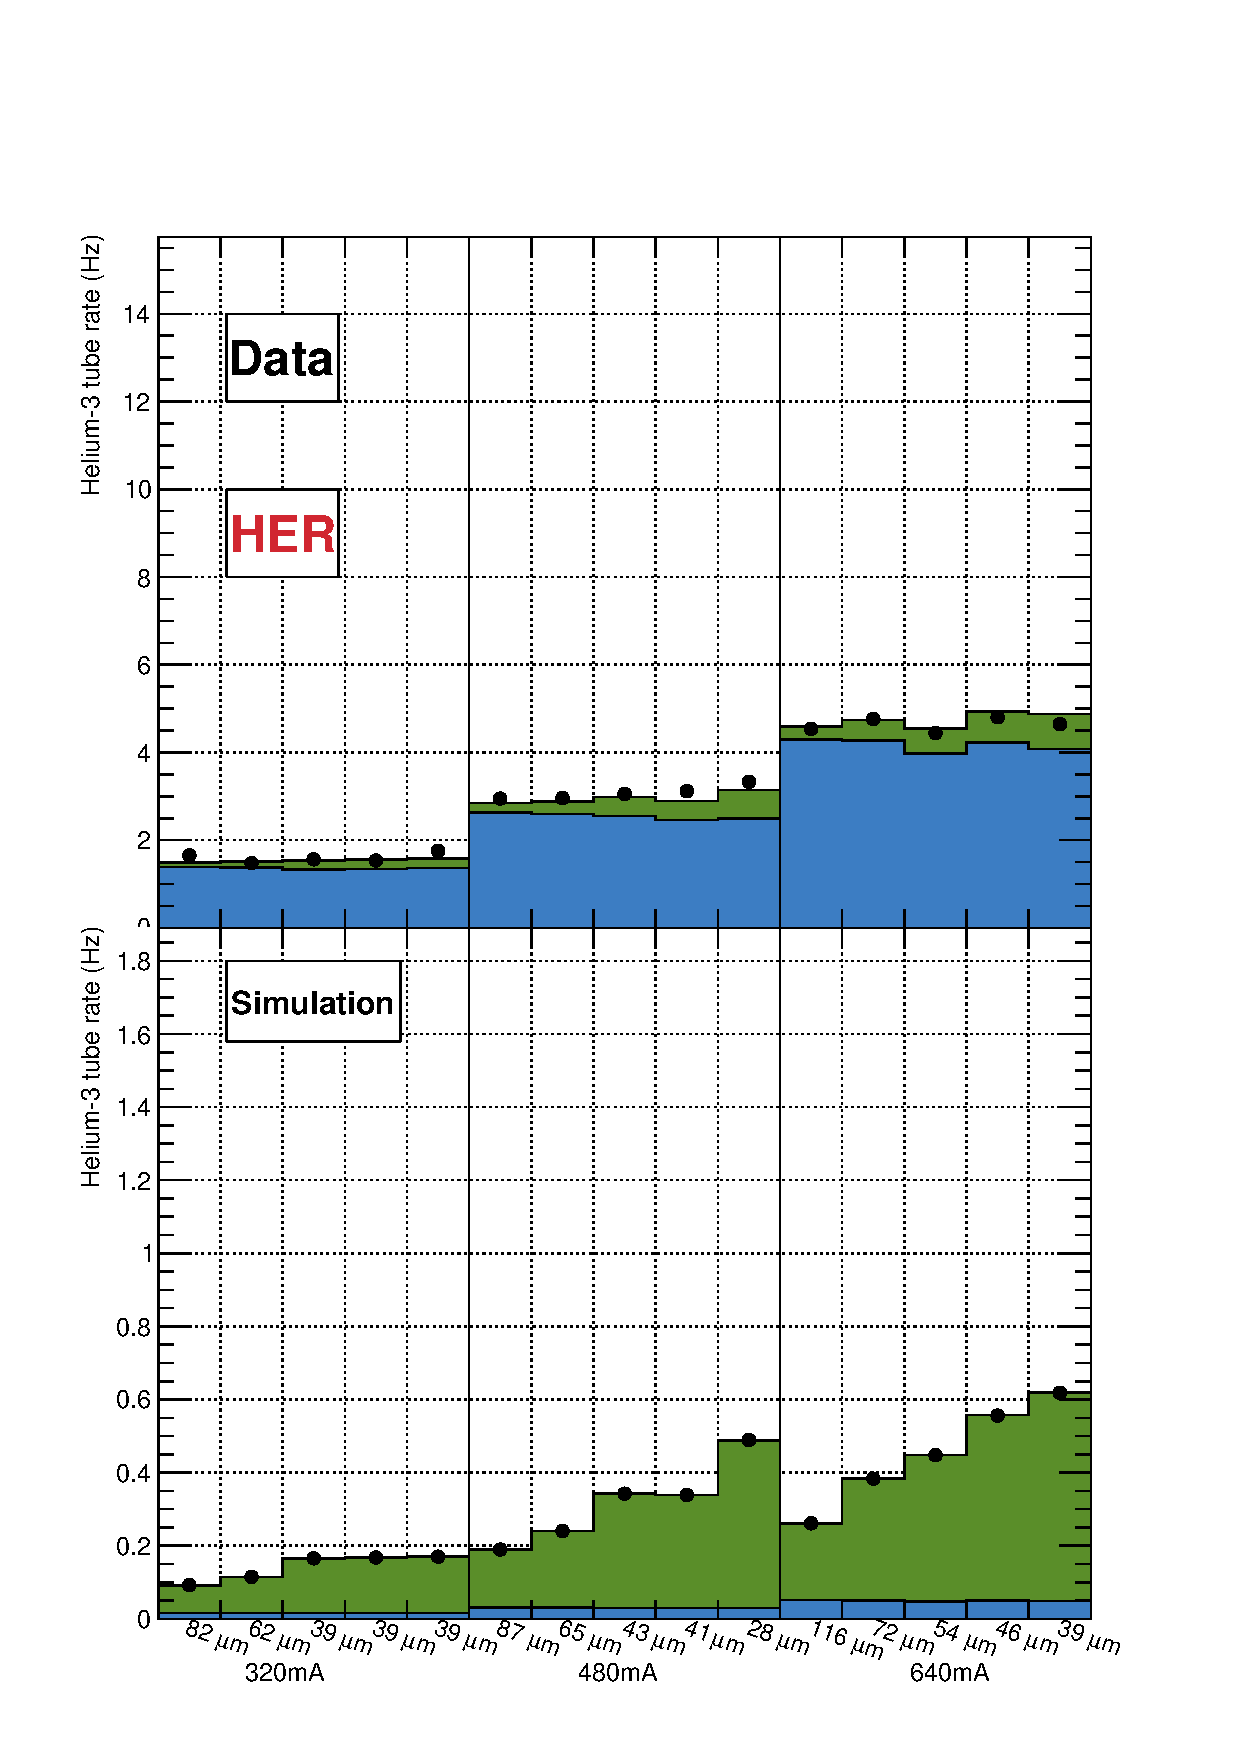
\includegraphics[width=\textwidth]{images/HERTousFirstPass_1}
		\begin{picture}(2,2)
			\put(-100,260){\thicklines\circle*{10}} %1
			\put(-120,240){\thicklines\circle{10}}  %2
			\put(-100,220){\thicklines\circle{10}}  %3
			\put(-80,240){\thicklines\circle{10}}   %0
			\put(-104, 237){$\phi$}  
		\end{picture}
	\caption[Result of fit for Touschek experiments, HER, channel 1]{Result of fit for Touschek experiments, HER, channel 1. Green is the beam-beam component, blue is the beam-gas component, and black is the rate measured in \he tube channel 1. Error bars are the standard deviation of the mean of the rate in that bin and are too small to be seen on this scale.}	
	\label{fig:HERTous11}
\end{figure}
\begin{figure}
	\centerfloat
		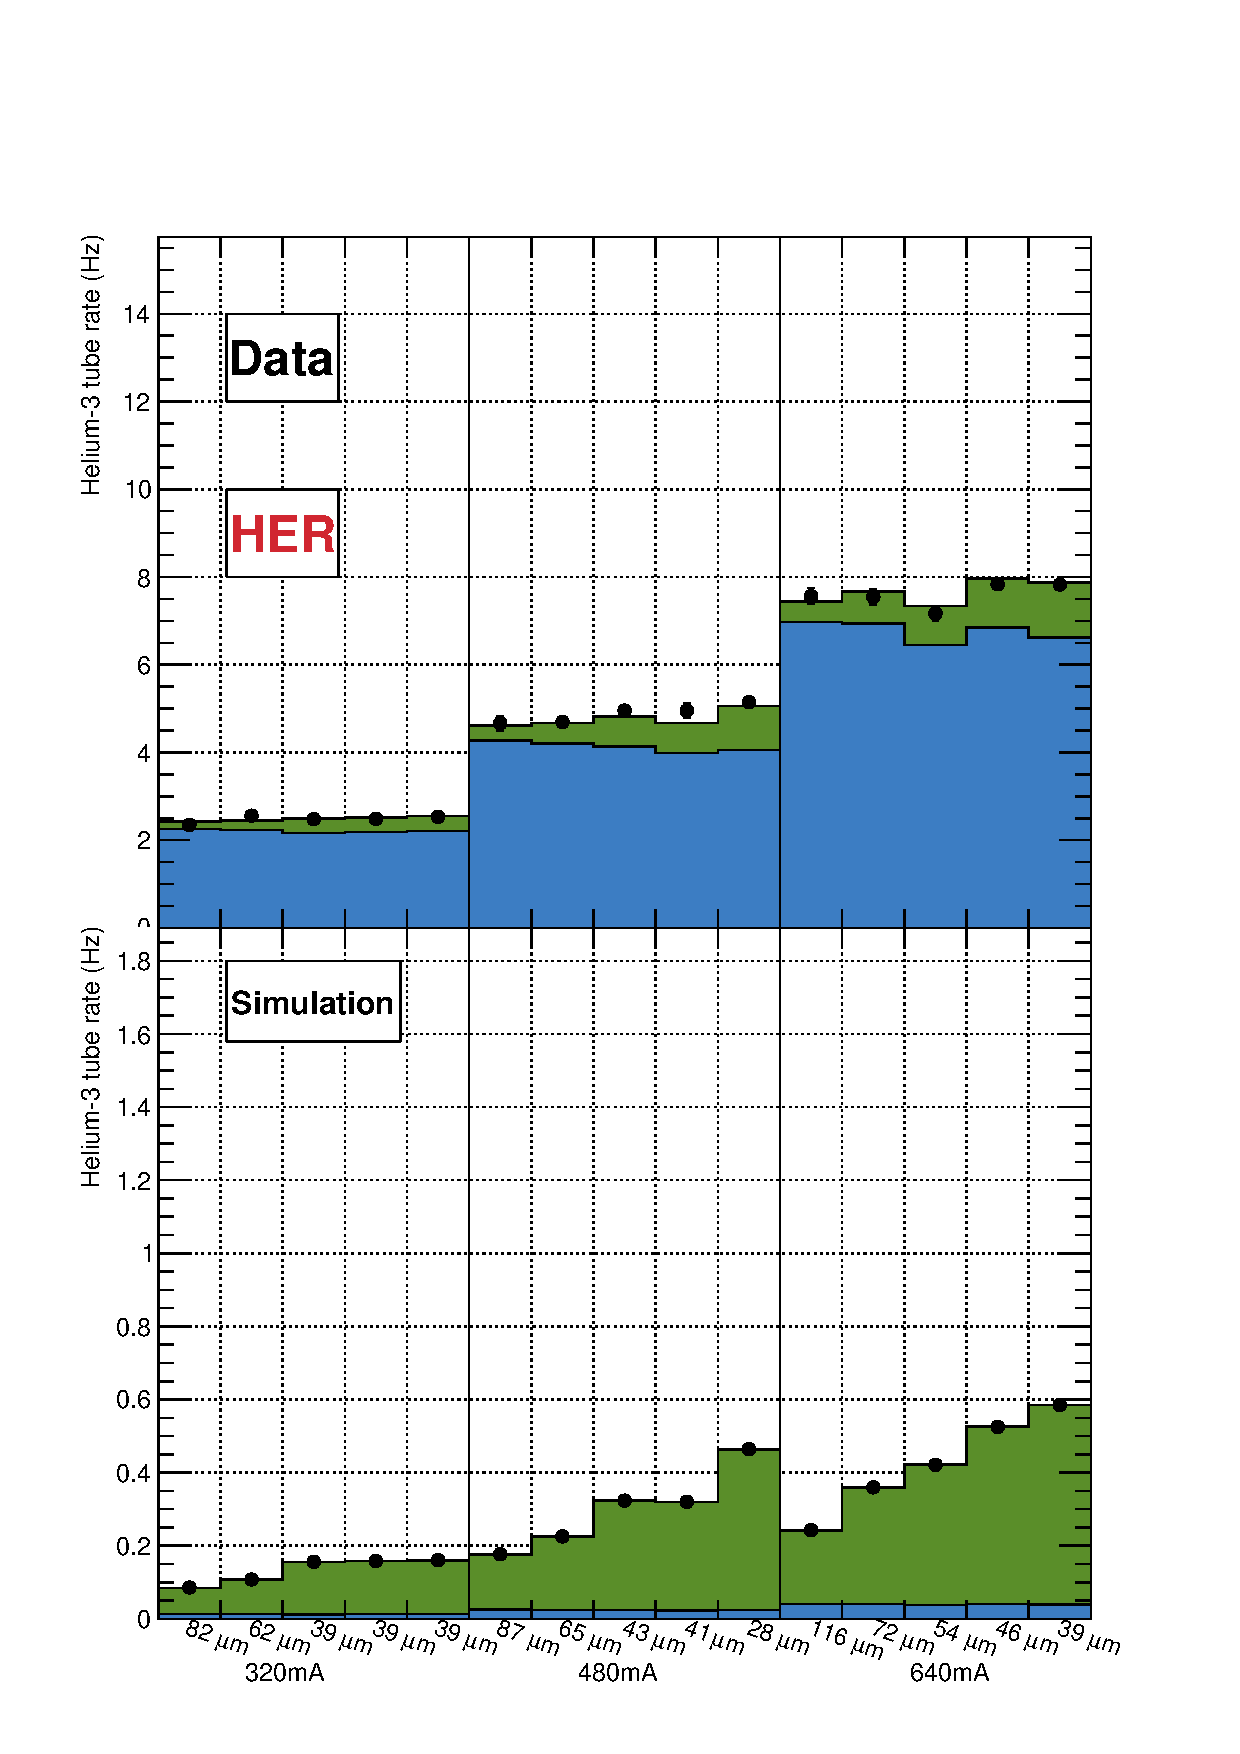
\includegraphics[width=\textwidth]{images/HERTousFirstPass_2}
		\begin{picture}(2,2)
			\put(-100,260){\thicklines\circle{10}} %1
			\put(-120,240){\thicklines\circle*{10}}  %2
			\put(-100,220){\thicklines\circle{10}}  %3
			\put(-80,240){\thicklines\circle{10}}   %0
			\put(-104, 237){$\phi$}  
		\end{picture}
	\caption[Result of fit for Touschek experiments, HER, channel 2]{Result of fit for Touschek experiments, HER, channel 2. Green is the beam-beam component, blue is the beam-gas component, and black is the rate measured in \he tube channel 2. Error bars are the standard deviation of the mean of the rate in that bin and are too small to be seen on this scale.}	
	\label{fig:HERTous12}
\end{figure}
\begin{figure}
	\centerfloat
		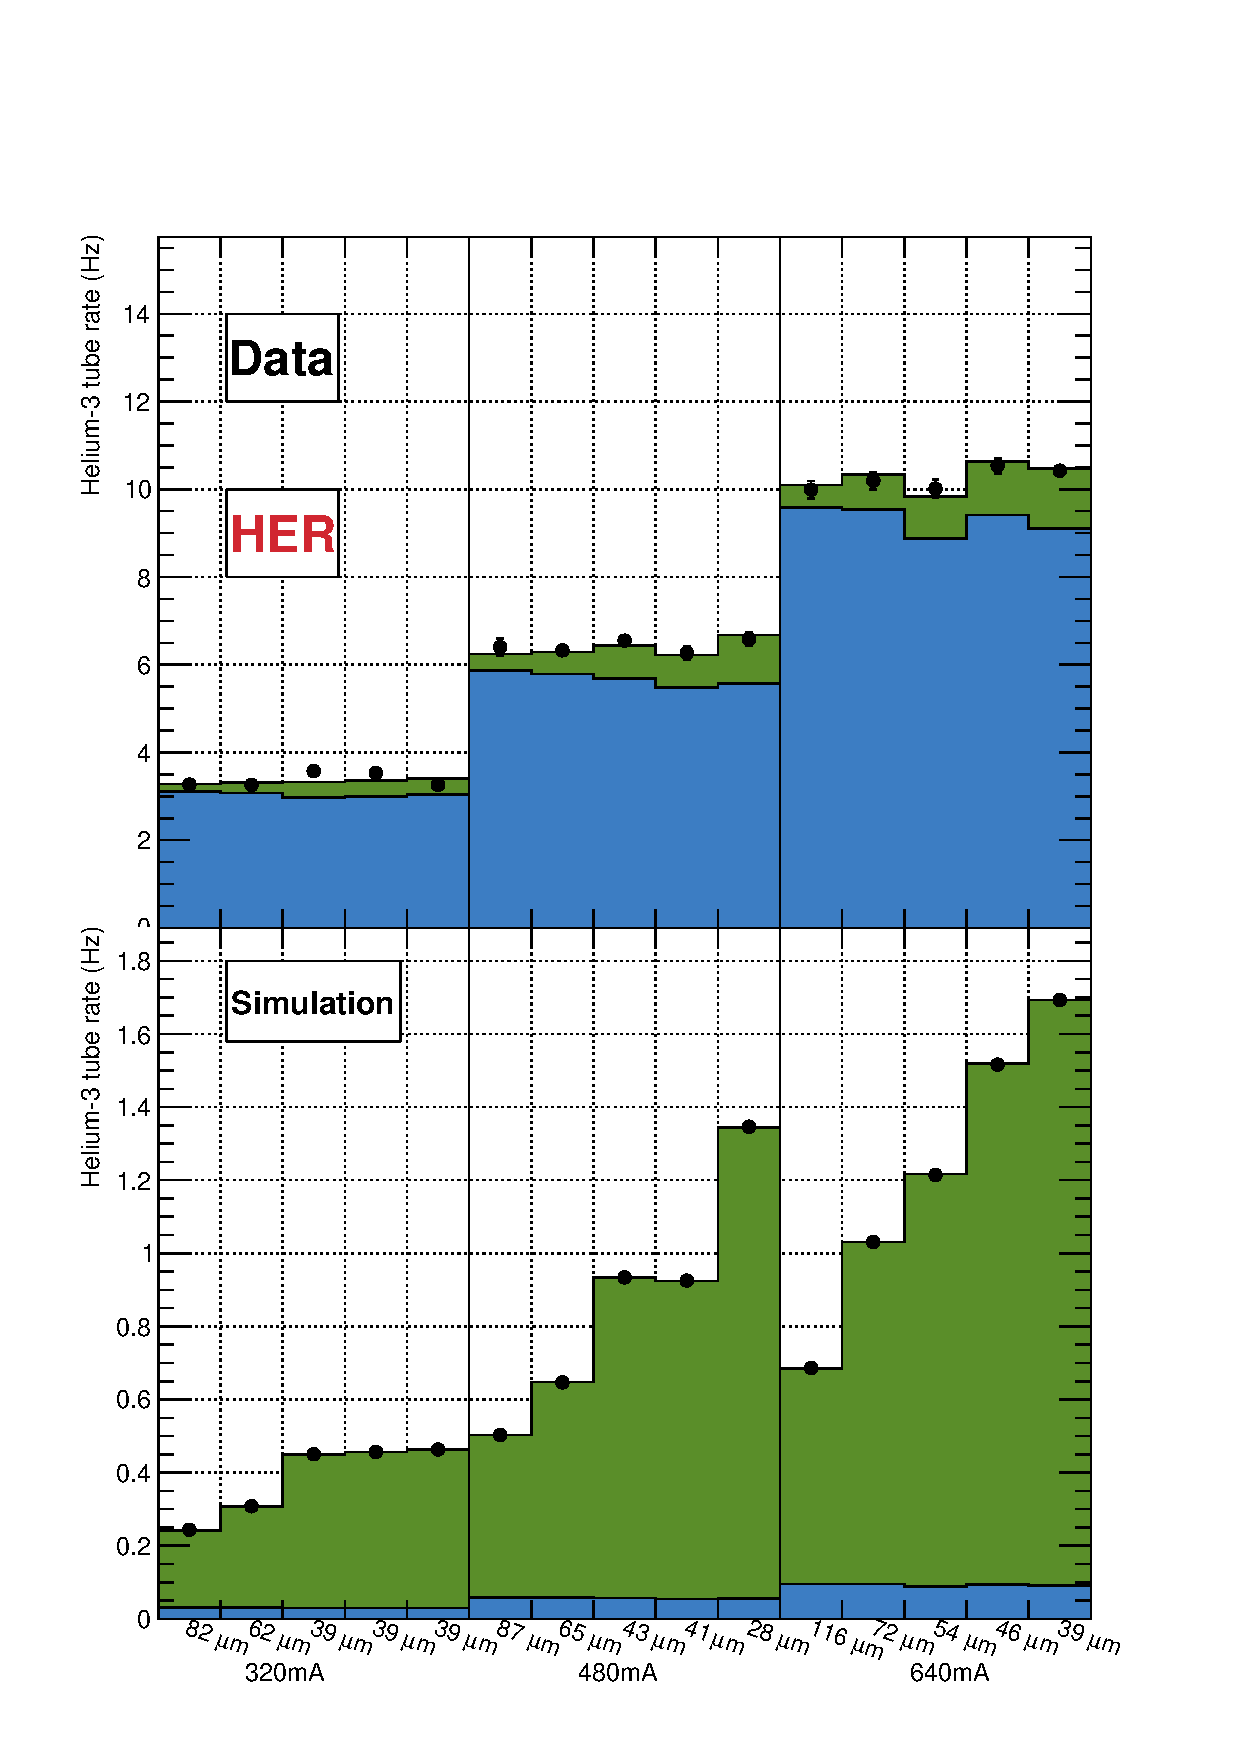
\includegraphics[width=\textwidth]{images/HERTousFirstPass_3}
		\begin{picture}(2,2)
			\put(-100,260){\thicklines\circle{10}} %1
			\put(-120,240){\thicklines\circle{10}}  %2
			\put(-100,220){\thicklines\circle*{10}}  %3
			\put(-80,240){\thicklines\circle{10}}   %0
			\put(-104, 237){$\phi$}  
		\end{picture}
	\caption[Result of fit for Touschek experiments, HER, channel 3]{Result of fit for Touschek experiments, HER, channel 3. Green is the beam-beam component, blue is the beam-gas component, and black is the rate measured in \he tube channel 3. Error bars are the standard deviation of the mean of the rate in that bin and are too small to be seen on this scale.}	
	\label{fig:HERTous13}
\end{figure}





As evident from Figs~\ref{fig:HERTous10} -~\ref{fig:HERTous13}, the simulation greatly underestimates the beam-gas component in the HER, and to a lesser extent in the LER. This is due to two factors: $Z_{\mathrm{eff}}$ is not known in the HER, and $P_{\mathrm{scale}}$ is not known in either beam. Using a value of 1 for these parameters does not give the correct beam-gas component. To compensate, the ratio of the beam-gas fit parameter, $c_{gas}$, to the Touschek fit parameter, $c_{T}$, for data is used to estimate a value for $P_{\mathrm{scale}}Z_{\mathrm{eff}}^{2}$ (or simply $P_{\mathrm{scale}}$ for the LER, since $Z$ is known) that is used in the weighting of the simulation:
\begin{equation}
	{P_{\mathrm{scale}}Z_{\mathrm{eff}}^{2} = \frac{\sum_{n=1}^{4}(c_{\mathrm{gas}}/c_{\mathrm{T}})_{i~\mathrm{data}}}{\sum_{n=1}^{4}(c_{\mathrm{gas}}/c_{\mathrm{T}})_{i~\mathrm{sim}}}}
\label{eqn:Pscale1}
\end{equation}
The motivation for this is that all the parameters of the Touschek component of the fit are relatively well known, while the pressure and $Z_{\mathrm{eff}}$ in the beam-gas component are not well known. The beam-gas to Touschek ratio in the data is used to determine $P_{\mathrm{scale}}Z_{\mathrm{eff}}^{2}$ to be used in the simulation weighting. Note that this does not constrain the overall total prediction of the background from the simulation or the absolute individual contributions.

\begin{table}[htb]
	\centering
	\begin{tabular}{ ccS }
	& $P_{\mathrm{scale}}$ (LER)	&	{$P_{\mathrm{scale}}Z_{\mathrm{eff}}^{2}$ (HER)}	\\	\hline \hline
0	&	0.980	&	122.07	\\	
1	&	0.853	&	73.45	\\	
2	&	1.019	&	88.62	\\	
3	&	0.962	&	115.10	\\	\hline
Combined (see Eqn~\ref{eqn:Pscale1})	&	0.950	&	96.27	\\	\hline

	\end{tabular}	
	\caption[$P_{\mathrm{scale}}$ and $P_{\mathrm{scale}}Z_{\mathrm{eff}}^{2}$ values]{$P_{\mathrm{scale}}$ and $P_{\mathrm{scale}}Z_{\mathrm{eff}}^{2}$ values.}
	\label{tab:PScaleZsq}
\end{table}

The values for $P_{\mathrm{scale}}Z_{\mathrm{eff}}^{2}$ can be found in Table~\ref{tab:PScaleZsq}. Note that the values are significantly different between LER and HER. This is because the $Z_{\mathrm{eff}}$ is known for the LER, but not the HER. 

The simulation was then re-weighted, and the data and simulation were again fit to Eqn~\ref{eqn:TousFit}. The results of the fit for LER and HER are shown in Figs~\ref{fig:LERTous20},~\ref{fig:LERTous21},~\ref{fig:LERTous22},~\ref{fig:LERTous23} and~\ref{fig:HERTous20},~\ref{fig:HERTous21},~\ref{fig:HERTous22},~\ref{fig:HERTous23}, respectively. The values of the fit parameters can be found in Table~\ref{tab:FitPars}.



\begin{figure}
	\centerfloat
		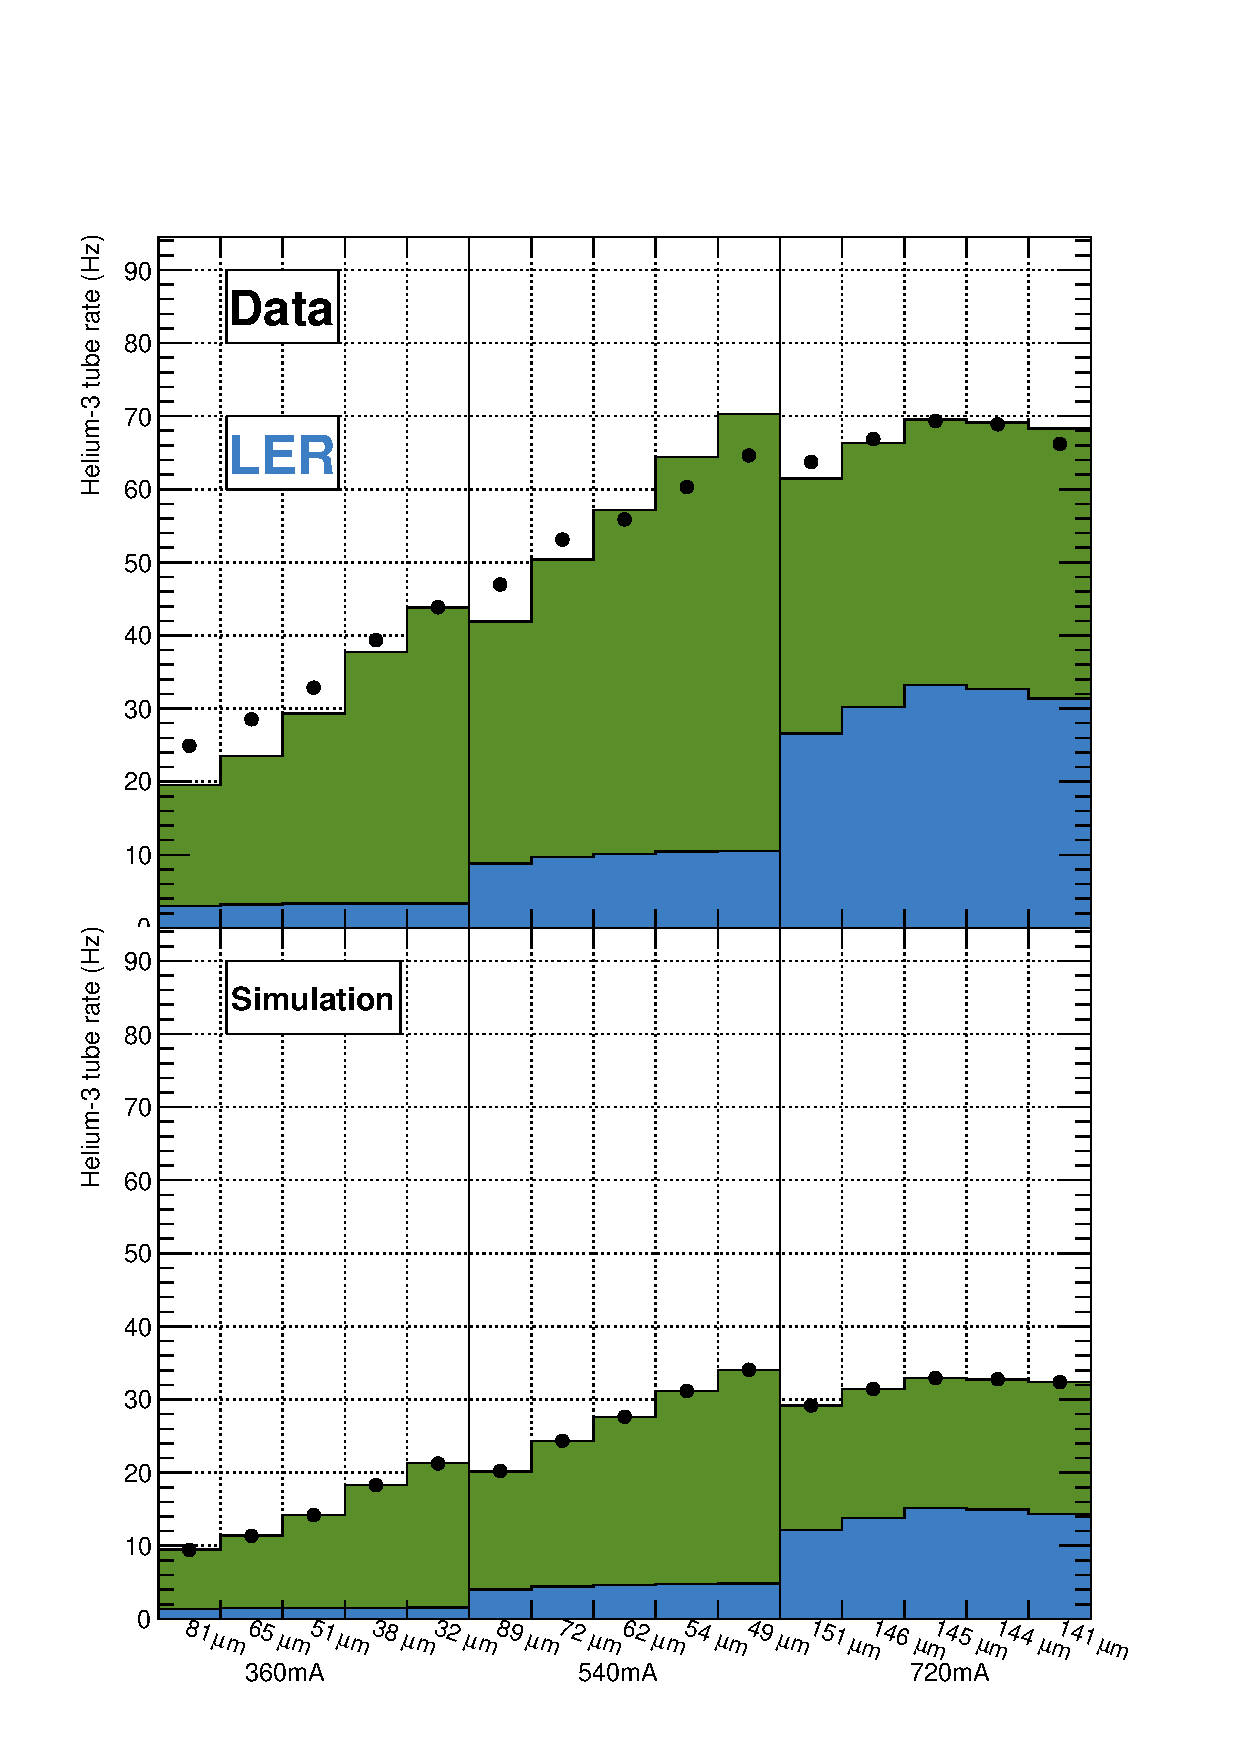
\includegraphics[width=\textwidth]{images/LERTousSecondPass_0}
		\begin{picture}(2,2)
			\put(-100,260){\thicklines\circle{10}}
			\put(-120,240){\thicklines\circle{10}}
			\put(-100,220){\thicklines\circle{10}}
			\put(-80,240){\thicklines\circle*{10}}
			\put(-104, 237){$\phi$}  
		\end{picture}
	\caption[Result of fit for Touschek experiments after simulation is weighted by $P_{\mathrm{scale}}$, LER, channel 0]{Result of fit for Touschek experiments after simulation is weighted by $P_{\mathrm{scale}}$, LER, channel 0. Green is the beam-beam component, blue is the beam-gas component, and black is the rate measured in \he tube channel 0. Error bars are the standard deviation of the mean of the rate in that bin and are too small to be seen on this scale.}	
	\label{fig:LERTous20}
\end{figure}

\begin{figure}
	\centerfloat
		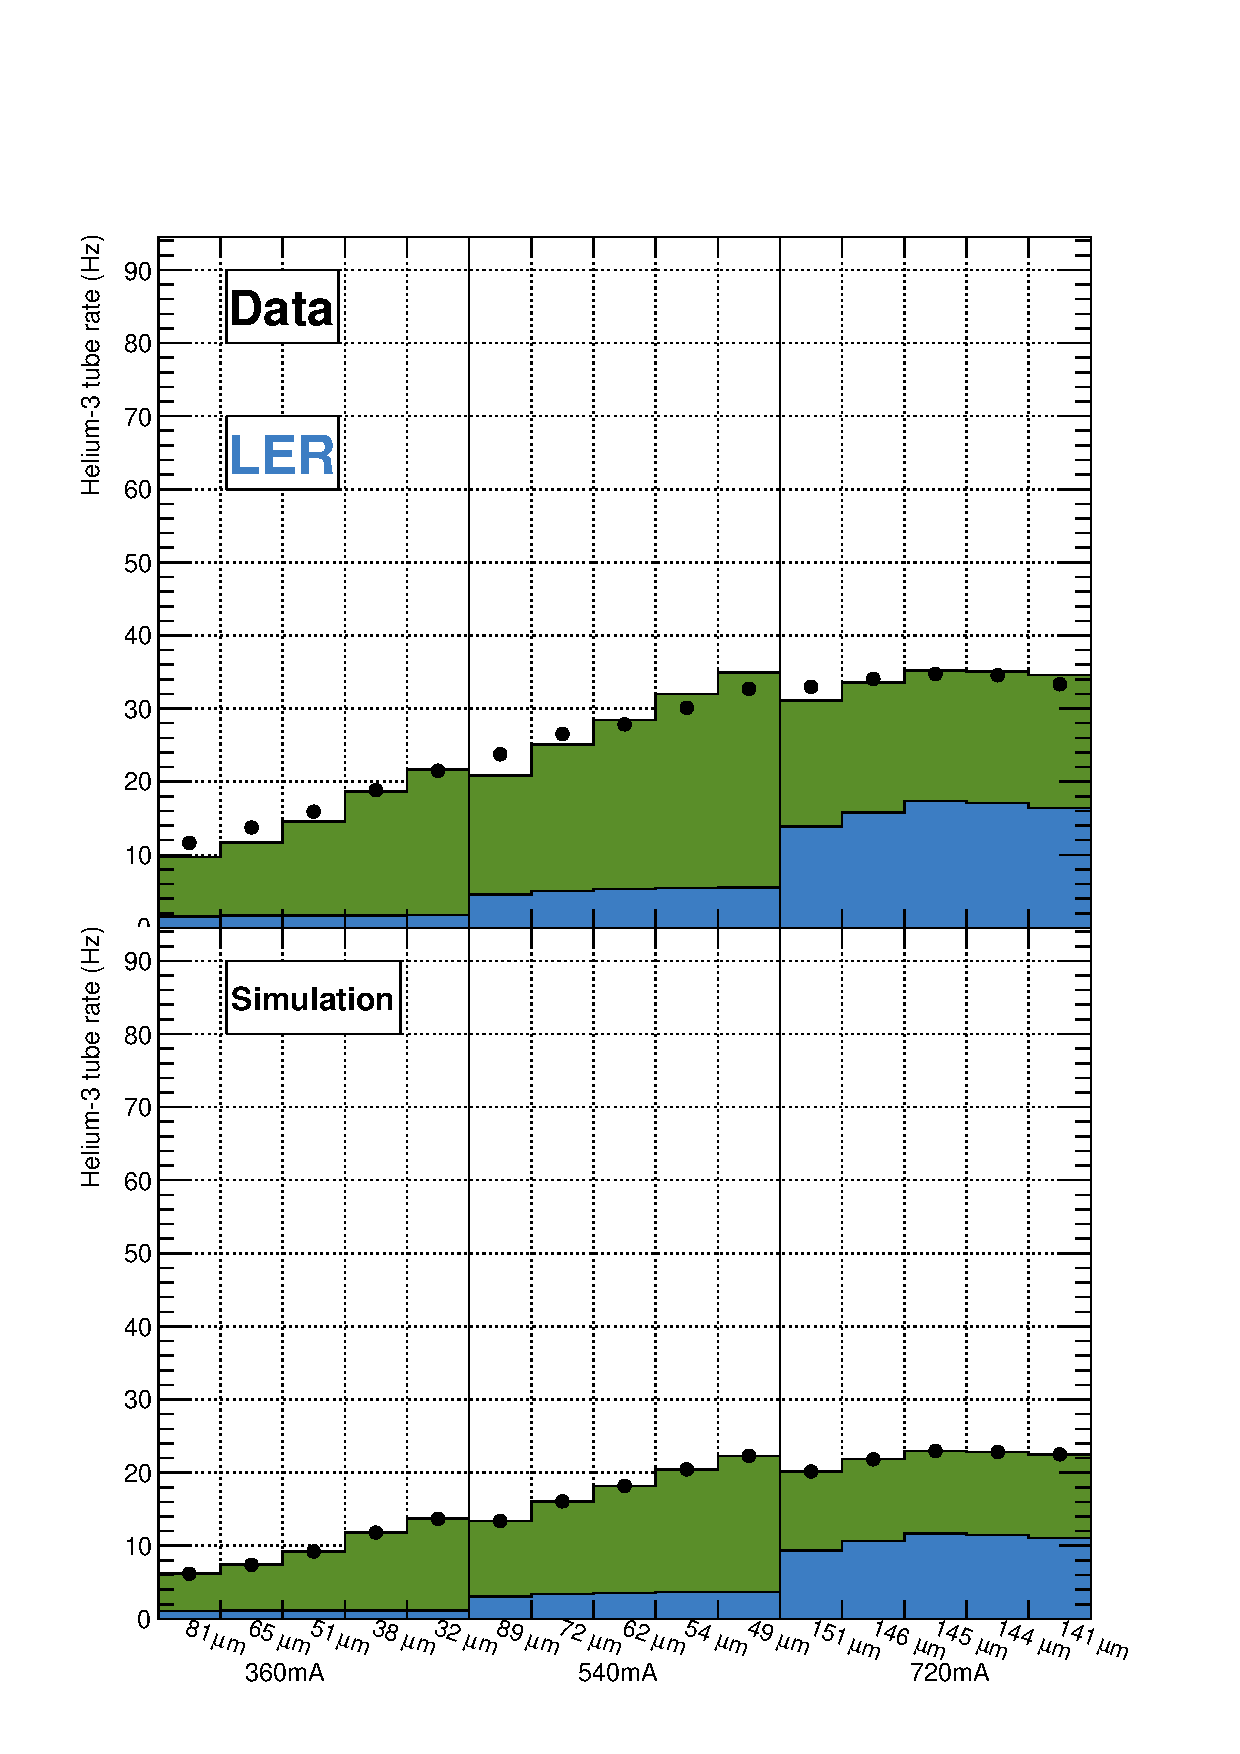
\includegraphics[width=\textwidth]{images/LERTousSecondPass_1}
		\begin{picture}(2,2)
			\put(-100,260){\thicklines\circle*{10}}
			\put(-120,240){\thicklines\circle{10}}
			\put(-100,220){\thicklines\circle{10}}
			\put(-80,240){\thicklines\circle{10}}
			\put(-104, 237){$\phi$}  
		\end{picture}
	\caption[Result of fit for Touschek experiments after simulation is weighted by $P_{\mathrm{scale}}$, LER, channel 1]{Result of fit for Touschek experiments after simulation is weighted by $P_{\mathrm{scale}}$, LER, channel 1. Green is the beam-beam component, blue is the beam-gas component, and black is the rate measured in \he tube channel 1. Error bars are the standard deviation of the mean of the rate in that bin and are too small to be seen on this scale.}	
	\label{fig:LERTous21}
\end{figure}

\begin{figure}
	\centerfloat
		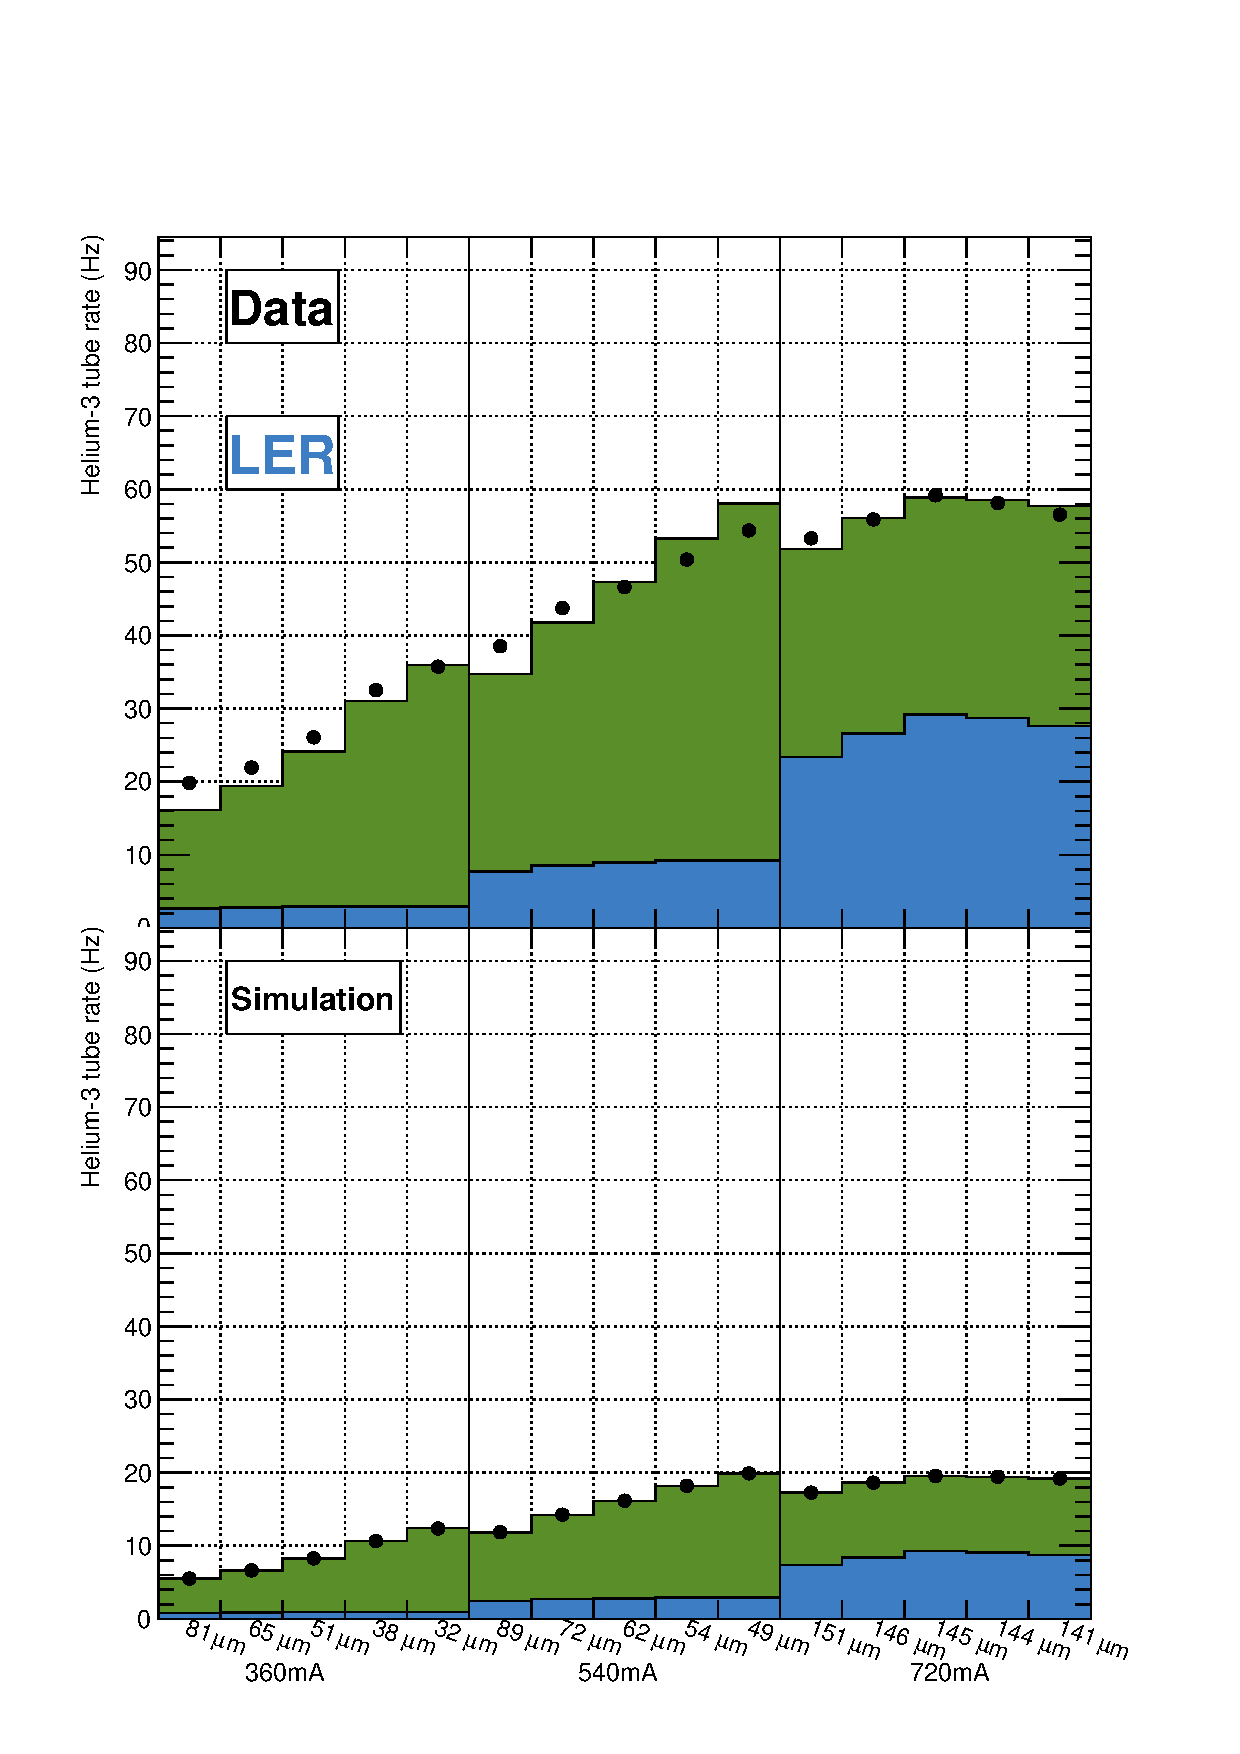
\includegraphics[width=\textwidth]{images/LERTousSecondPass_2}
		\begin{picture}(2,2)
			\put(-100,260){\thicklines\circle{10}}
			\put(-120,240){\thicklines\circle*{10}}
			\put(-100,220){\thicklines\circle{10}}
			\put(-80,240){\thicklines\circle{10}}
			\put(-104, 237){$\phi$}  
		\end{picture}
	\caption[Result of fit for Touschek experiments after simulation is weighted by $P_{\mathrm{scale}}$, LER, channel 2]{Result of fit for Touschek experiments after simulation is weighted by $P_{\mathrm{scale}}$, LER, channel 2. Green is the beam-beam component, blue is the beam-gas component, and black is the rate measured in \he tube channel 2. Error bars are the standard deviation of the mean of the rate in that bin and are too small to be seen on this scale.}	
	\label{fig:LERTous22}
\end{figure}

\begin{figure}
	\centerfloat
		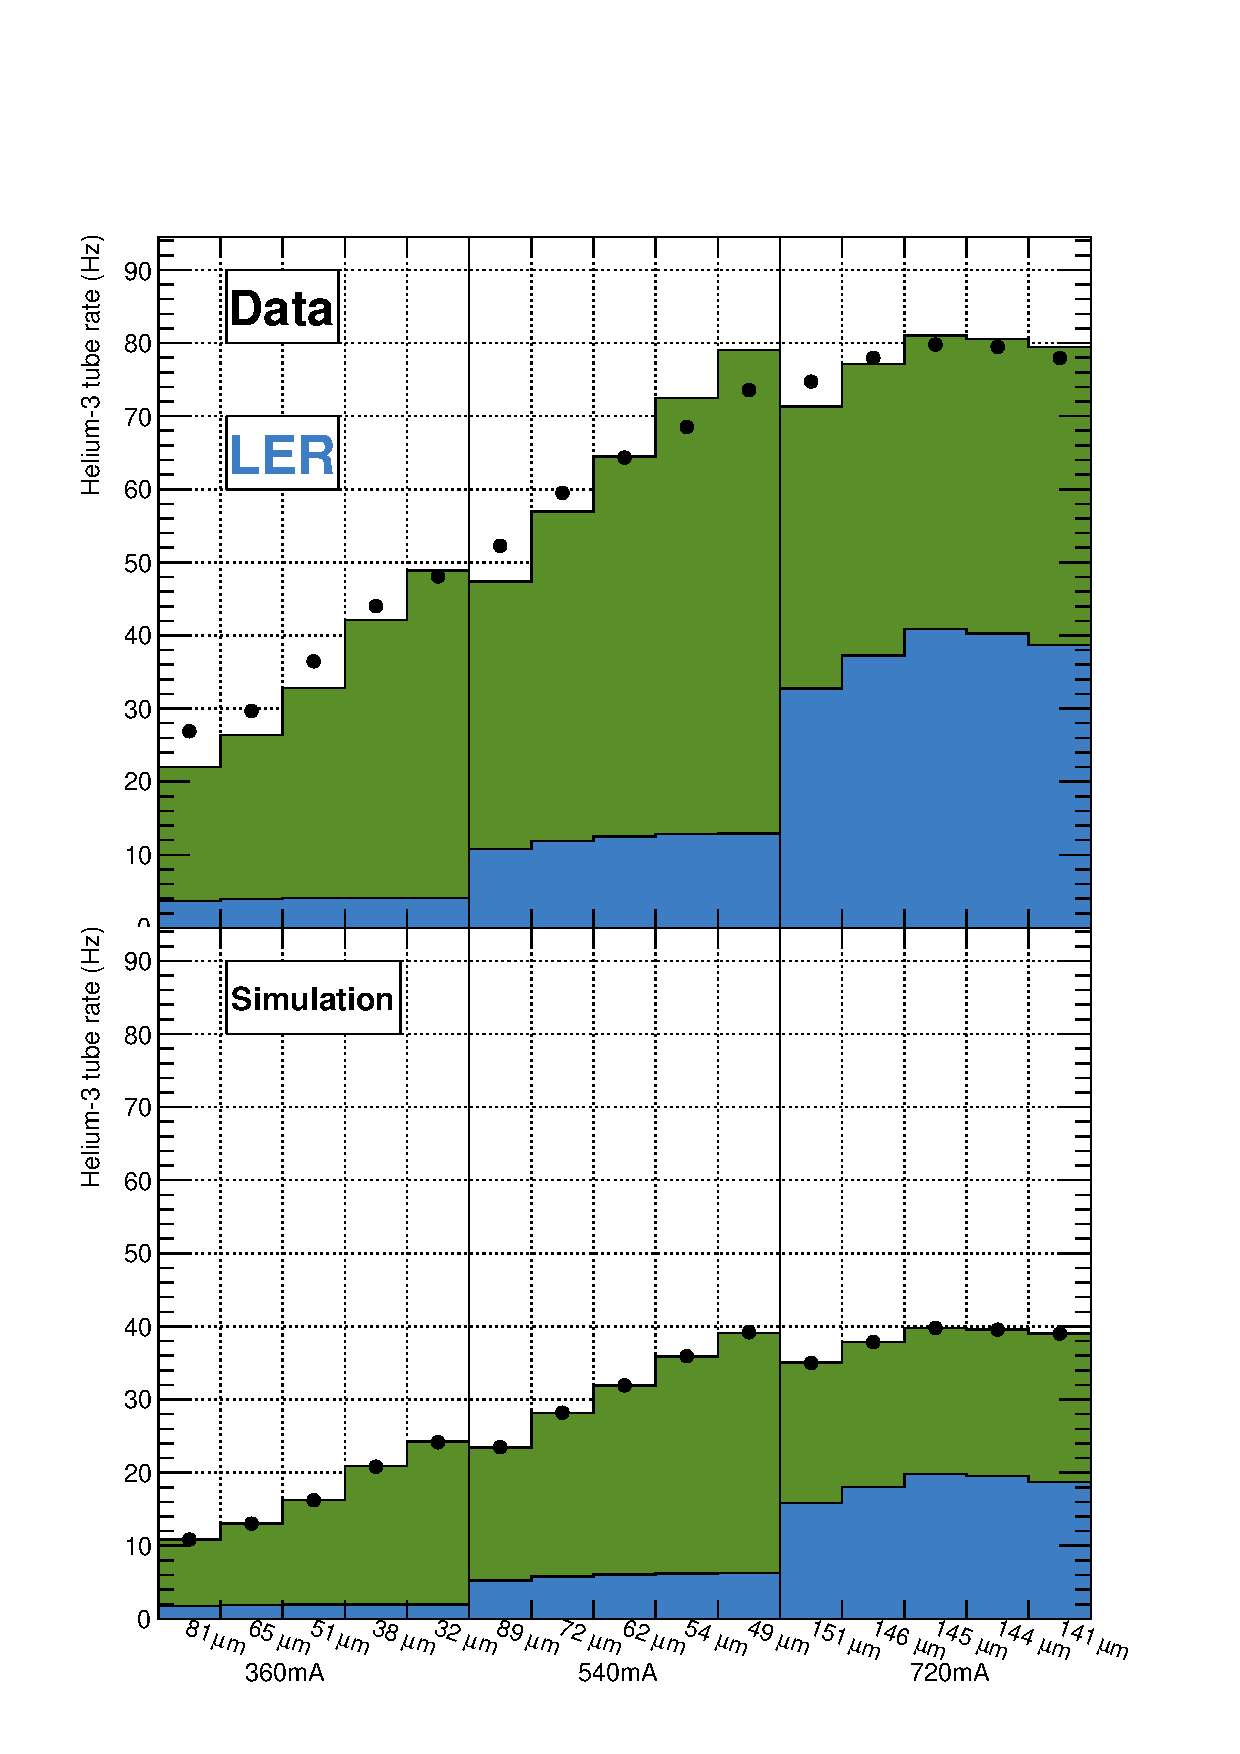
\includegraphics[width=\textwidth]{images/LERTousSecondPass_3}
		\begin{picture}(2,2)
			\put(-100,260){\thicklines\circle{10}}
			\put(-120,240){\thicklines\circle{10}}
			\put(-100,220){\thicklines\circle*{10}}
			\put(-80,240){\thicklines\circle{10}}
			\put(-104, 237){$\phi$}  
		\end{picture}
	\caption[Result of fit for Touschek experiments after simulation is weighted by $P_{\mathrm{scale}}$, LER, channel 3]{Result of fit for Touschek experiments after simulation is weighted by $P_{\mathrm{scale}}$, LER, channel 3. Green is the beam-beam component, blue is the beam-gas component, and black is the rate measured in \he tube channel 3. Error bars are the standard deviation of the mean of the rate in that bin and are too small to be seen on this scale.}	
	\label{fig:LERTous23}
\end{figure}


\begin{figure}
	\centerfloat
		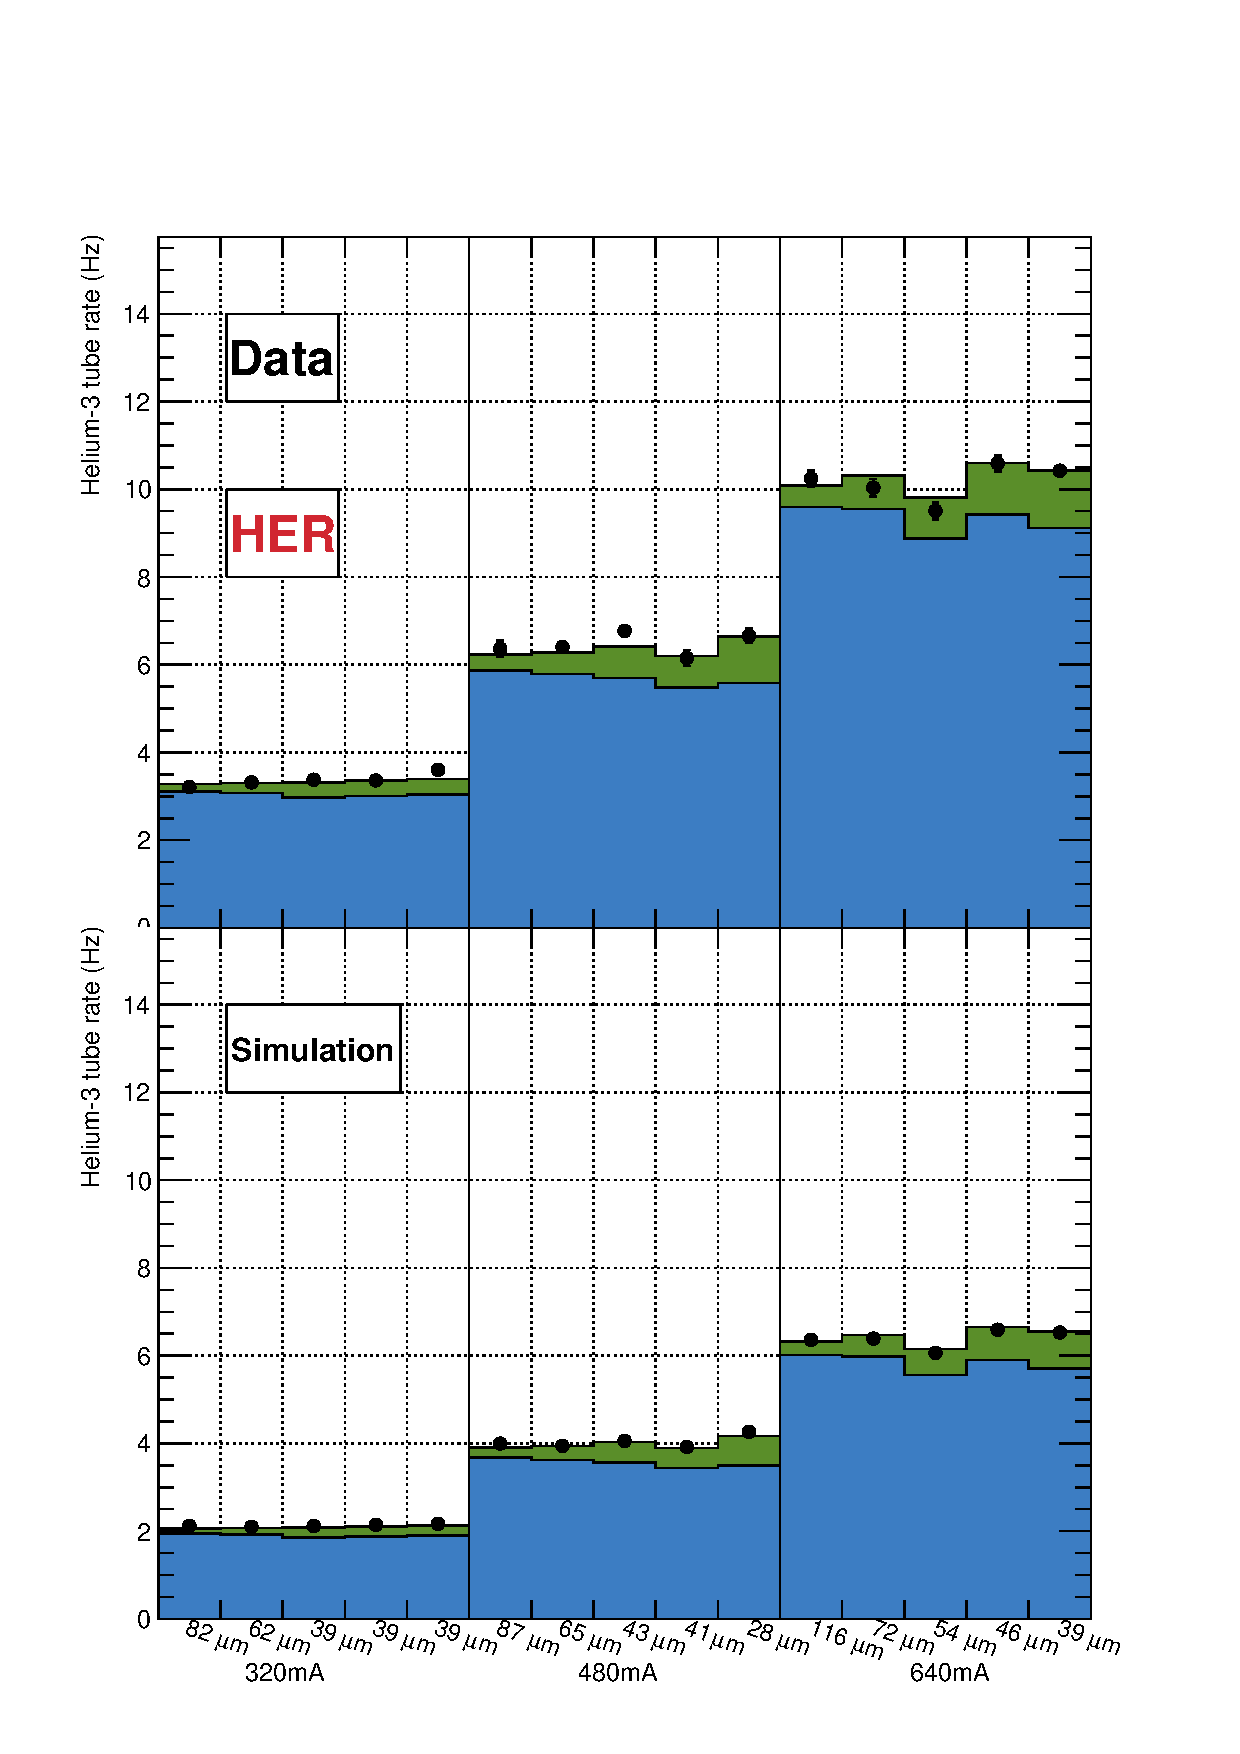
\includegraphics[width=\textwidth]{images/HERTousSecondPass_0}
		\begin{picture}(2,2)
			\put(-100,260){\thicklines\circle{10}} %1
			\put(-120,240){\thicklines\circle{10}}  %2
			\put(-100,220){\thicklines\circle{10}}  %3
			\put(-80,240){\thicklines\circle*{10}}   %0
			\put(-104, 237){$\phi$}  
		\end{picture}
	\caption[Result of fit for Touschek experiments after simulation is weighted by $P_{\mathrm{scale}}Z_{\mathrm{eff}}^{2}$, HER, channel 0]{Result of fit for Touschek experiments after simulation is weighted by $P_{\mathrm{scale}}Z_{\mathrm{eff}}^{2}$ , HER, channel 0. Green is the beam-beam component, blue is the beam-gas component, and black is the rate measured in \he tube channel 0. Error bars are the standard deviation of the mean of the rate in that bin and are too small to be seen on this scale.}	
	\label{fig:HERTous20}
\end{figure}

\begin{figure}
	\centerfloat
		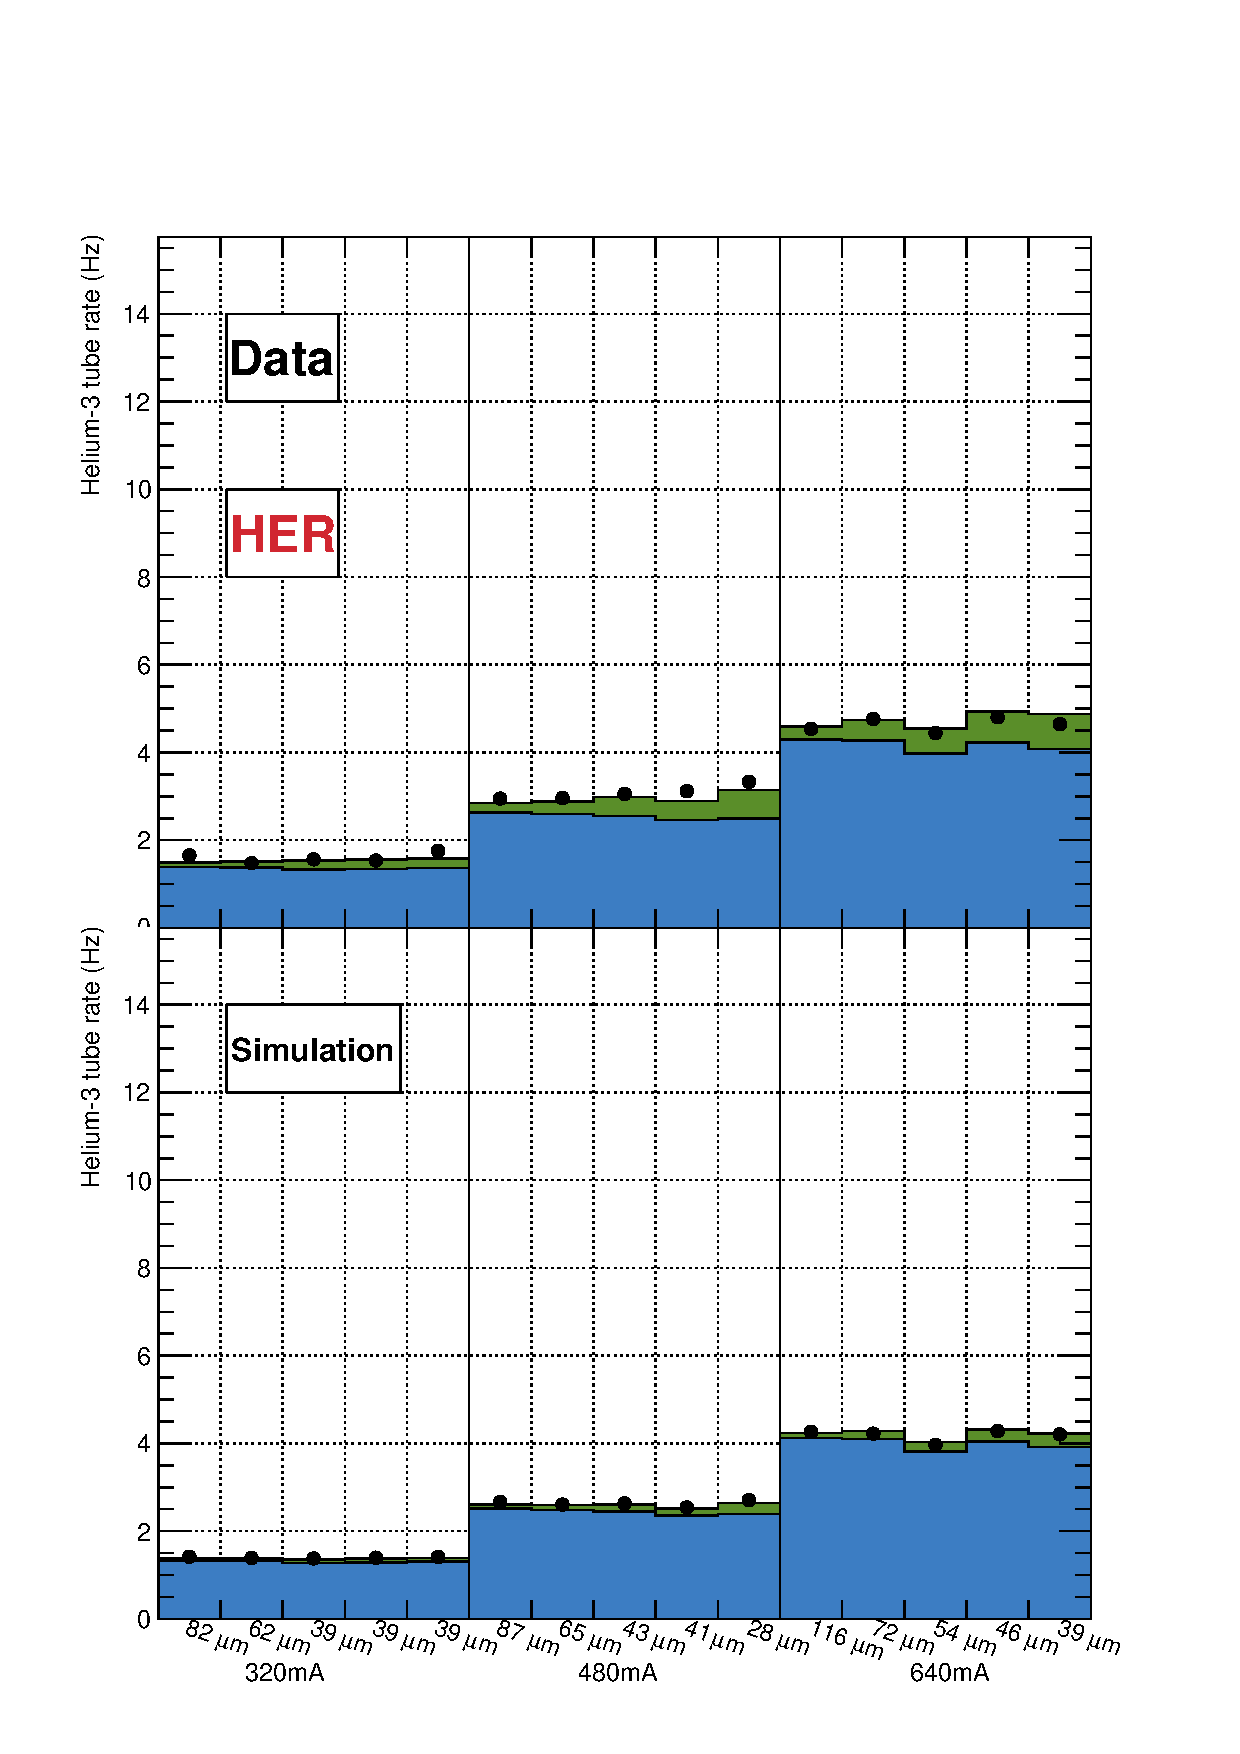
\includegraphics[width=\textwidth]{images/HERTousSecondPass_1}
		\begin{picture}(2,2)
			\put(-100,260){\thicklines\circle*{10}} %1
			\put(-120,240){\thicklines\circle{10}}  %2
			\put(-100,220){\thicklines\circle{10}}  %3
			\put(-80,240){\thicklines\circle{10}}   %0
			\put(-104, 237){$\phi$}  
		\end{picture}
	\caption[Result of fit for Touschek experiments after simulation is weighted by $P_{\mathrm{scale}}Z_{\mathrm{eff}}^{2}$, HER, channel 1]{Result of fit for Touschek experiments after simulation is weighted by $P_{\mathrm{scale}}Z_{\mathrm{eff}}^{2}$ , HER, channel 1. Green is the beam-beam component, blue is the beam-gas component, and black is the rate measured in \he tube channel 1. Error bars are the standard deviation of the mean of the rate in that bin and are too small to be seen on this scale.}	
	\label{fig:HERTous21}
\end{figure}

\begin{figure}
	\centerfloat
		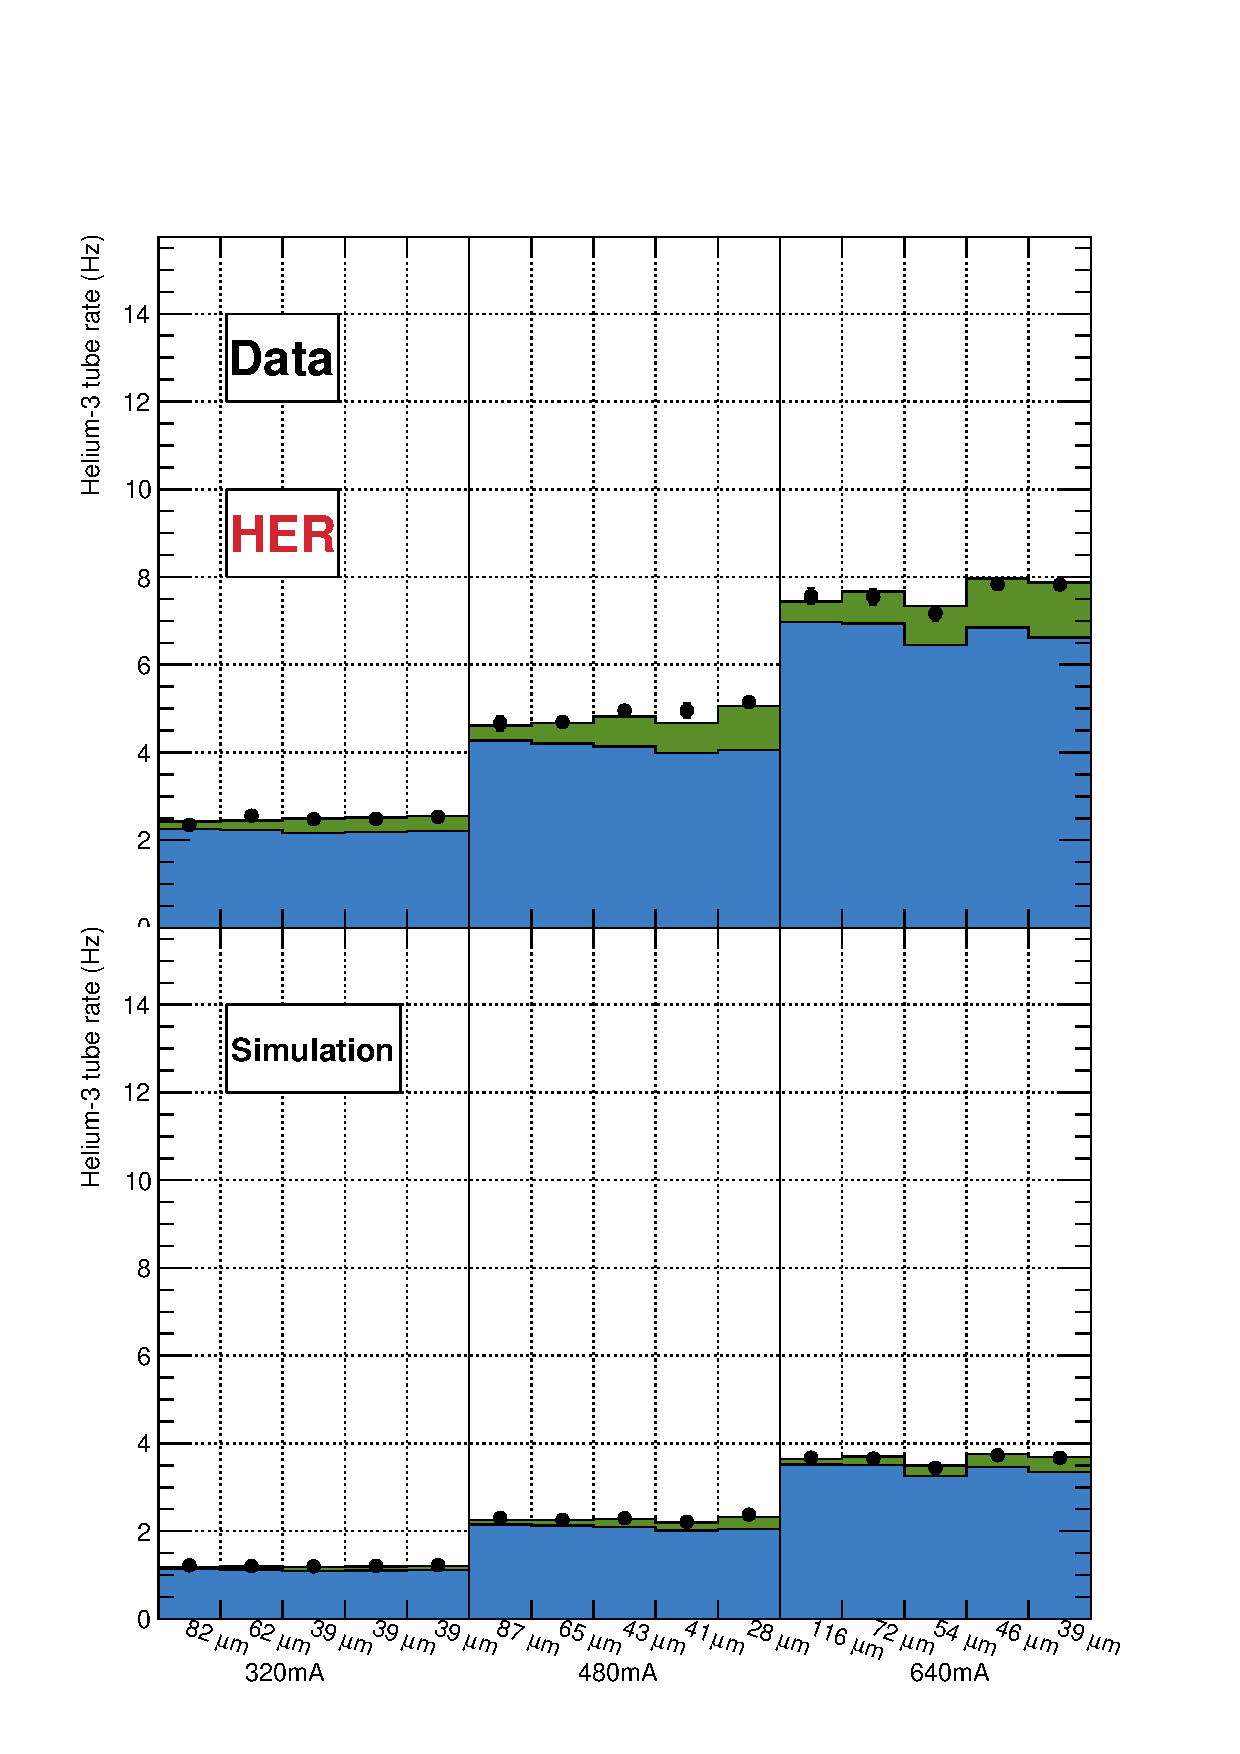
\includegraphics[width=\textwidth]{images/HERTousSecondPass_2}
		\begin{picture}(2,2)
			\put(-100,260){\thicklines\circle{10}} %1
			\put(-120,240){\thicklines\circle*{10}}  %2
			\put(-100,220){\thicklines\circle{10}}  %3
			\put(-80,240){\thicklines\circle{10}}   %0
			\put(-104, 237){$\phi$}  
		\end{picture}
	\caption[Result of fit for Touschek experiments after simulation is weighted by $P_{\mathrm{scale}}Z_{\mathrm{eff}}^{2}$, HER, channel 2]{Result of fit for Touschek experiments after simulation is weighted by $P_{\mathrm{scale}}Z_{\mathrm{eff}}^{2}$ , HER, channel 2. Green is the beam-beam component, blue is the beam-gas component, and black is the rate measured in \he tube channel 2. Error bars are the standard deviation of the mean of the rate in that bin and are too small to be seen on this scale.}	
	\label{fig:HERTous22}
\end{figure}

\begin{figure}
	\centerfloat
		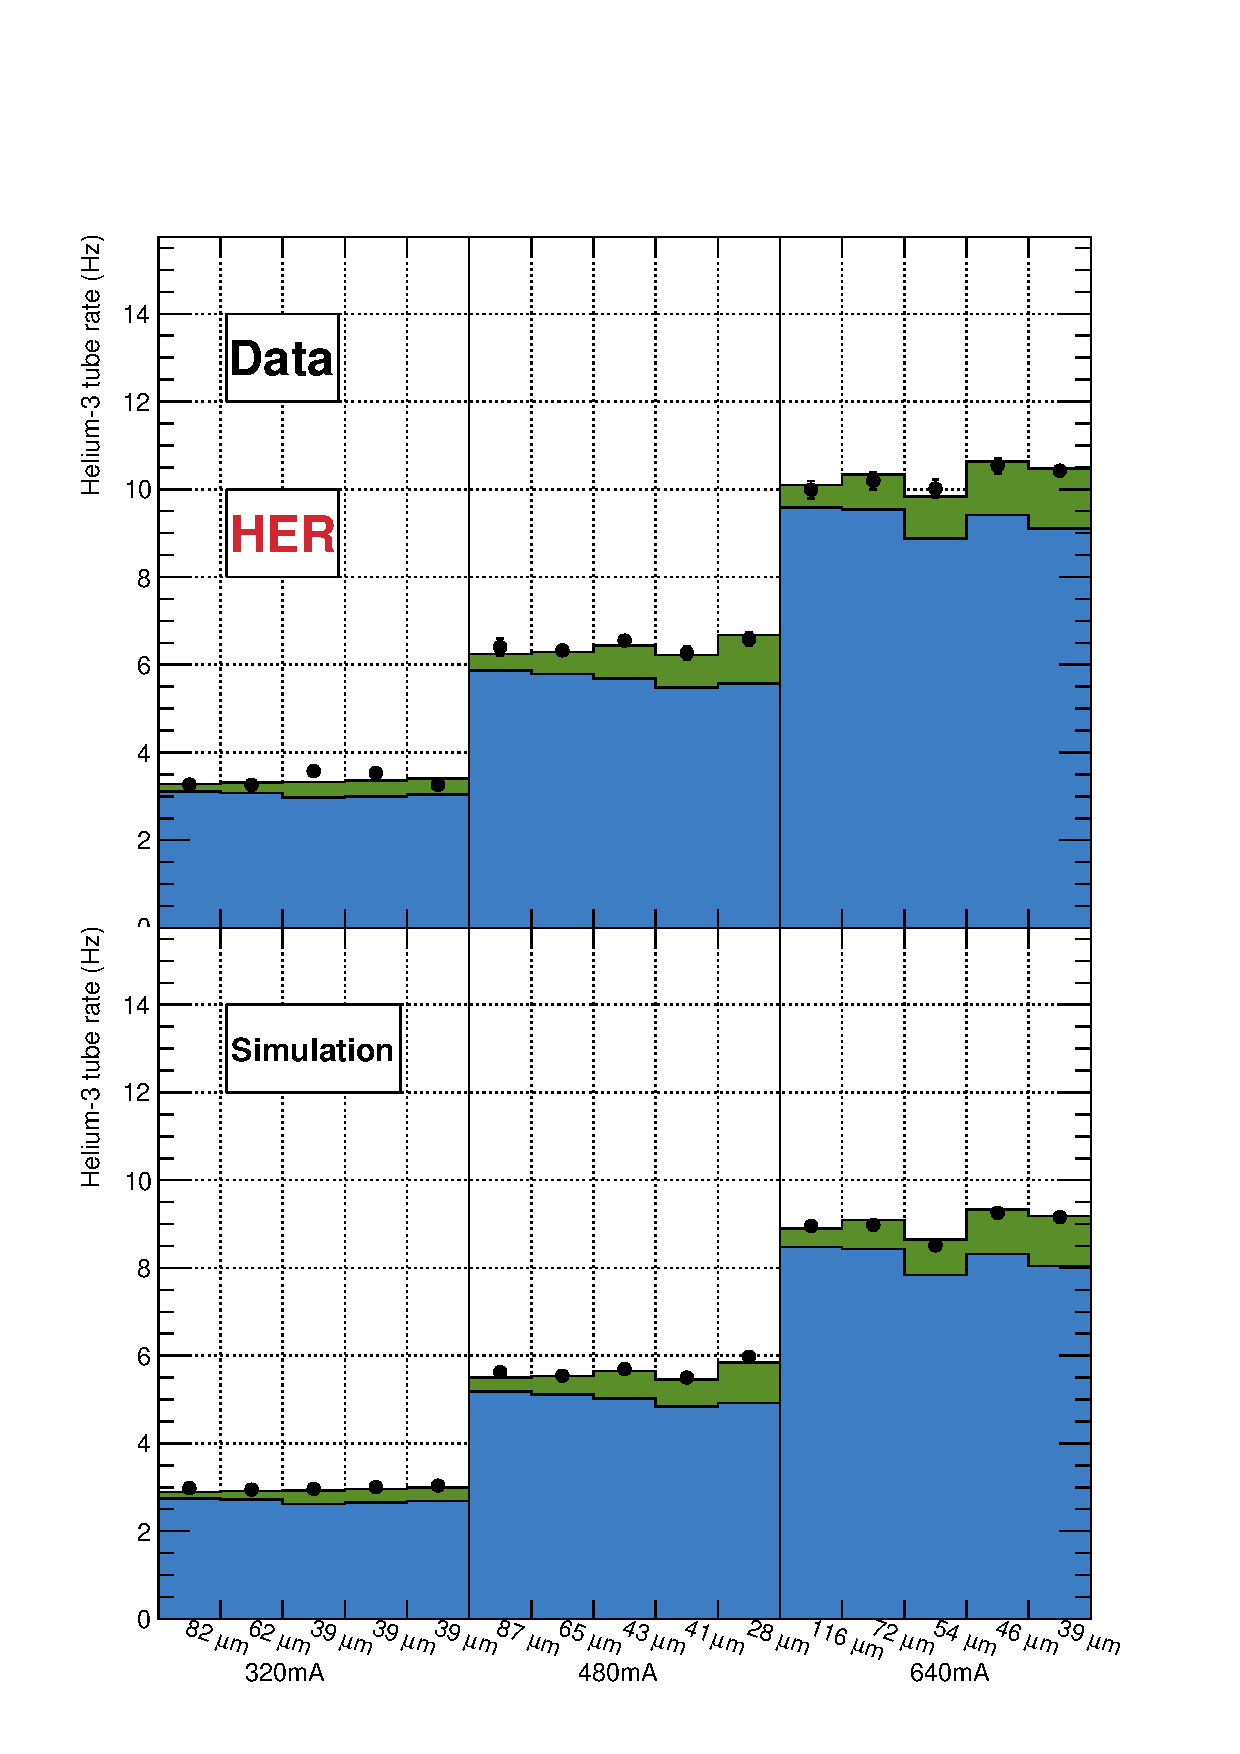
\includegraphics[width=\textwidth]{images/HERTousSecondPass_3}
		\begin{picture}(2,2)
			\put(-100,260){\thicklines\circle{10}} %1
			\put(-120,240){\thicklines\circle{10}}  %2
			\put(-100,220){\thicklines\circle*{10}}  %3
			\put(-80,240){\thicklines\circle{10}}   %0
			\put(-104, 237){$\phi$}  
		\end{picture}
	\caption[Result of fit for Touschek experiments after simulation is weighted by $P_{\mathrm{scale}}Z_{\mathrm{eff}}^{2}$, HER, channel 3]{Result of fit for Touschek experiments after simulation is weighted by $P_{\mathrm{scale}}Z_{\mathrm{eff}}^{2}$ , HER, channel 3. Green is the beam-beam component, blue is the beam-gas component, and black is the rate measured in \he tube channel 3. Error bars are the standard deviation of the mean of the rate in that bin and are too small to be seen on this scale.}	
	\label{fig:HERTous23}
\end{figure}





	In order to verify the overall accuracy of the simulation, a ratio of the data to simulation for the beam-gas and Touschek parameters is defined:
\begin{subequations}
\begin{align}
		{(D/S)_{\mathrm{gas}} = c_{\mathrm{gas}}^{\mathrm{data}}/c_{\mathrm{gas}}^{\mathrm{sim}}} \\
		{(D/S)_{\mathrm{T}} = c_{\mathrm{T}}^{\mathrm{data}}/c_{\mathrm{T}}^{\mathrm{sim}}}
\end{align}
\end{subequations}
where $(D/S)_{\mathrm{gas}}$ is the data to simulation ratio for beam-gas, and $(D/S)_{\mathrm{T}}$ is the data to simulation ratio for Touschek.

The more accurate the simulation, the closer these ratios will be to 1. These ratios can also be used to scale the simulation to better match the data. The values of these ratios can be found in Table~\ref{tab:dataSimRatio}. Note that the table omits the uncertainty on the ratio. This is discussed in detail in \S~\ref{sec:Systematics}.

\begin{table}[htb]
	\centering
	\begin{tabular}{ ccc }
		& $(D/S)_{\mathrm{T}}$	&  $(D/S)_{\mathrm{gas}}$	\\ \hline \hline
	LER	& 2.153		& 2.188	\\ 
	HER	& 1.905		& 1.319	\\ \hline 
	\end{tabular}
	\caption[Ratio of data to simulation for beam-gas and Touschek parameters]{Ratio of data to simulation for beam-gas and Touschek parameters.}
	\label{tab:dataSimRatio}
\end{table}

\subsection{Systematic Uncertainties in Touschek Experiments}
\label{sec:Systematics}


	In order to get the uncertainty on $(D/S)_{gas}$ and $(D/S)_{T}$, it is necessary to determine the uncertainty on the beam current, beam size, $P_{\mathrm{scale}}Z_{\mathrm{eff}}^{2}$, and the \he tube efficiencies used in the simulation.

\paragraph{Uncertainty on beam current}
	
	The beam current is known to quite a high level of precision. The uncertainty on the current does not depend on the current, and is estimated to be 0.03~mA \cite{HiroEmailCurrentError}.


\paragraph{Uncertainty on beam size}
	
	The distribution of the beam size for HER and LER during the beam size scans is shown in Fig~\ref{fig:BeamSizeError}. To estimate the uncertainty on the beam size, the distributions are fit to Gaussian functions. The mean and sigma of the fits can be found in Table~\ref{tab:beamSizeGausFits}. For the HER, the uncertainty on the beam size is estimated to be 3.71\%. For the LER, the beam size uncertainty is estimated to be 1.37\%.


\begin{figure}
	\centering
	\subfigure{
		\begin{overpic}[trim={0 0 0 0.75cm},clip, width=\textwidth]{images/LERBeamSize}
		\end{overpic}
		\label{fig:LERBeamSizeError}
	}
	\subfigure{
		\begin{overpic}[trim={0 0 0 0.75cm},clip, width=\textwidth]{images/HERBeamSize}
		\end{overpic}
		\label{fig:HERBeamSizeError}
	}
	\caption[Estimation of beam size uncertainty]{Estimation of beam size uncertainty. Measurements were taken from the X-ray beam size monitor during beam size scans. The different colours indicate different subruns.}	
	\label{fig:BeamSizeError}
\end{figure}


\begin{table}[htb]
	\centering
	\begin{tabular}{ lllll }
		& Colour in Fig~\ref{fig:BeamSizeError}	& mean ($\mu m$)	& $\sigma$ ($\mu m$) & $\sigma$/mean	\\ \hline \hline
	LER	& Grey	& 81.02$\pm$0.10	& 1.30$\pm$0.09	    	& 0.0161	\\
		& Green	& 65.20$\pm$0.06	& 0.77$\pm$0.05	    	& 0.0114	\\ \hline
	HER	& Grey	& 86.96$\pm$0.23	& 3.19$\pm$0.23	    	& 0.0367	\\
		& Red	& 41.84$\pm$0.07	& 1.56$\pm$0.05	    	& 0.0372	\\
		& Blue	& 28.18$\pm$0.07    	& 1.06$\pm$0.05	& 0.0375	\\ \hline
	\end{tabular}
	\caption[Fit parameters for beam size distributions]{Fit parameters for beam size distributions.}
	\label{tab:beamSizeGausFits}
\end{table}


\paragraph{Uncertainty on $P_{\mathrm{s}}$$_{\mathrm{c}}$$_{\mathrm{a}}$$_{\mathrm{l}}$$_{\mathrm{e}}$$Z$$_{\mathrm{e}}^2$$_{\mathrm{f}}$$_{\mathrm{f}}$}

	The value of $P_{\mathrm{scale}}Z_{\mathrm{eff}}^{2}$ is calculated by averaging over the four \he tubes. To estimate the uncertainty, this parameter is calculated separately for each tube (see Table~\ref{tab:PScaleZsq}). The RMS of the four values is used as the uncertainty. These values can be found in Table~\ref{tab:PscaleZUncertainy}

\begin{table}[htb]
	\centering
	\begin{tabular}{ lSS }
		& {$P_{\mathrm{scale}}Z_{\mathrm{eff}}^{2}$}	& {RMS of $P_{\mathrm{scale}}Z_{\mathrm{eff}}^{2}$}	\\ \hline \hline
	HER	& 96.27	& 22.7	 \\
	LER	& 0.950	& 0.071 \\ \hline
	\end{tabular}
	\caption[RMS of $P_{\mathrm{scale}}Z_{\mathrm{eff}}^{2}$]{RMS of $P_{\mathrm{scale}}Z_{\mathrm{eff}}^{2}$.}
	\label{tab:PscaleZUncertainy}
\end{table}

\paragraph{Uncertainty on \He Tube Efficiency}

	The total uncertainty for each \he tube given in Table~\ref{tab:he3Calib} is used as the uncertainty on the \he tube efficiency.

\paragraph{Estimating the Uncertainty on $(D/S)$}

To estimate the systematic uncertainty from beam current, beam size, $P_{\mathrm{scale}}Z_{\mathrm{eff}}^{2}$, and \he tube efficiency, the simulation was re-weighted with each quantity separately adjusted to +1$\sigma$ and -1$\sigma$ values. The full analysis was then redone. For example:
\begin{subequations}
\begin{align}
		{I\rightarrow I+0.03\mathrm{~mA}} \\
		{I\rightarrow I-0.03\mathrm{~mA}}
\end{align}
\end{subequations}
and similarly for $\sigma_{y}$, $P_{\mathrm{scale}}$Z$^{2}$, and the \he tube efficiency. The analysis described in \S~\ref{sec:TousExp} was repeated to get new values of $R_{gas}$ and $R_{T}$. These are used to calculate the systematic error for each quantity:
\begin{subequations}
\begin{align}
	{\sigma_{(D/S)_{\mathrm{T}}+}^{I} = (D/S)_{\mathrm{T}}|_{I=I+0.03\mathrm{~mA}} - (D/S)_{\mathrm{T}}|_{\mathrm{nominal}}} \\
	{\sigma_{(D/S)_{\mathrm{T}}-}^{I} = (D/S)_{\mathrm{T}}|_{\mathrm{nominal}} - (D/S)_{\mathrm{T}}|_{I=I-0.03\mathrm{~mA}} }
\end{align}
\end{subequations}

Figure~\ref{fig:RatioWithErrors} shows the systematic uncertainty produced by each parameter. Table~\ref{tab:RatioWithErrors} contains the numerical values of these uncertainties. The uncertainty associated with $\phi$ is the standard deviation of the mean of the ratio for each of the four \he tubes, which are located at different $\phi$ positions around the beampipe. It is therefore a measure of how well the simulation predicts the $\phi$ distribution of the neutron flux.

\begin{table}[htb]
	\centering
	\begin{tabular}{ cSSSS }
	&	\multicolumn{2}{c}{Touschek}			&	\multicolumn{2}{c}{Beam-Gas}			\\	\hline \hline
LER	&	$\sigma_{+}$	&	$\sigma_{-}$	&	$\sigma_{+}$	&	$\sigma_{-}$	\\	
$P_{\mathrm{scale}}$	&	0.00084	&	0.00084	&	0.18	&	0.15	\\	
$\sigma_{y}$	&	0.028	&	0.028	&	0.	&	0.	\\	
I	&	0.00032	&	0.00032	&	0.000086	&	0.000086	\\	
$\phi$	&	0.27	&	0.27	&	0.35	&	0.35	\\	
$\varepsilon_{^3\mathrm{He}}$	&	0.21	&	0.18	&	0.21	&	0.18	\\	\hline
Total	&	0.34	&	0.33	&	0.44	&	0.42	\\	\hline
HER	&	$\sigma_{+}$	&	$\sigma_{-}$	&	$\sigma_{+}$	&	$\sigma_{-}$	\\	
$P_{\mathrm{scale}}Z^2$	&	0.24	&	0.19	&	0.41	&	0.25	\\	
$\sigma_{y}$	&	0.037	&	0.036	&	0.	&	0.	\\	
I	&	0.00018	&	0.00018	&	0.000076	&	0.000076	\\	
$\phi$	&	0.39	&	0.39	&	0.21	&	0.27	\\	
$\varepsilon_{^3\mathrm{He}}$	&	0.29	&	0.21	&	0.20	&	0.14	\\	\hline
Total	&	0.54	&	0.48	&	0.50	&	0.40	\\	\hline


	\end{tabular}
	\caption[Uncertainty contribution to $(D/S)$ from sources of systematic errors]{Uncertainty contribution to $(D/S)$ from sources of systematic errors. The values of (D/S) are given in Table~\ref{tab:dataSimRatio}.}
	\label{tab:RatioWithErrors}
\end{table}

\begin{figure}
	\centering
	\subfigure{
		\begin{overpic}[width=\textwidth]{images/LERRatioPlot}
		\end{overpic}
		\label{fig:LERRatioErrors}
	}
	\subfigure{
		\begin{overpic}[width=\textwidth]{images/HERRatioPlot}
		\end{overpic}
		\label{fig:HERRatioErrors}
	}
	\caption[LER and HER data simulation ratios with systematic errors]{LER and HER data simulation ratios with systematic errors. Blue is the beam-gas ratio, green is the Touschek ratio.}	
	\label{fig:RatioWithErrors}
\end{figure}

	The total uncertainty shown in Table~\ref{tab:RatioWithErrors} is the sum in quadrature of the uncertainty from each separate component. The major contributor to the uncertainty on the data/simulation ratio is the uncertainty due to the tubes being at different $\phi$ locations. This uncertainty is associated with the difference between the measured and simulated neutron flux at each different \he tube. A large uncertainty here shows that the simulation is incorrectly predicting the $\phi$ dependency of the neutron flux.


%------------------------------------------------------------------------------------------------

\subsection{Summary}

As shown in Tables~\ref{tab:dataSimRatio} and~\ref{tab:RatioWithErrors}, the ratio of data to simulation with uncertainties in the LER is 2.18$^{+0.44}_{-0.42}$ for beam-gas and 2.15$^{+0.34}_{-0.33}$ for Touschek, and in the HER is 1.32$^{+0.56}_{-0.36}$ for beam-gas and 1.91$^{+0.54}_{-0.48}$ for Touschek. The beam-gas LER-HER difference is $\pm2\sigma$, and the Touschek LER-HER difference is $\pm1\sigma$. Using these values, it is possible to re-scale the full Belle~II simulation to estimate what the neutron flux will actually be in Belle~II. This is discussed in Chapter~\ref{chap:Conseqences}.






















